\chapter{The Hypothesis and Knowledge graph}
\textit{
As defined in the introduction, a task consists of obstacles with corresponding target positions, an obstacle with an accompanying target position is called a subtask. The \textbf{hypothesis graph} contains nodes corresponding to obstacles at a certain position and edges corresponding to actions which relocate obstacles, and connect nodes in the hypothesis graph. A formal description of the hypothesis graph with its nodes and edges is given in \cref{subsec:hgraph_definition} and \cref{subsec:sys_iden_and_control_methods} elaborates the meaning of actions taken when traversing over one of the hypothesis graphs edges.\\
\newline
For every subtask in a task, a start and a target node is created, the hypothesis graph tries to connect the starting node to the corresponding target node by adding nodes and edges. The choice and content of these nodes and edges is based on local planning and randomisation, elaborated in~\cref{subsec:estimating_path_existence,subsec:motion_planning,subsec:manipulation_planning}. A successive path from a starting node to the corresponding target node is called a hypothesis. During the search for a hypothesis, the hypothesis graph resides in the \textbf{search loop}, when traversing over edges toward the target node the hypothesis graph resides in the \textbf{execution loop}, both loops are elaborated in \cref{subsec:2_loops}. When the hypothesis graph traverses over an edge, fault detectors monitors the progress, elaborated in \cref{subsec:fault_detection}. Finally an example of an hypothesis graph is given in \cref{subsec:hgraph_example}.\\
\newline
After execution, the traversed edge enters a review period, during which performance is checked in various metrics. The review is stored in a database, called the \textbf{knowledge graph} which serves to collect edges and rank them based on performance. The knowledge graph is defined in \cref{subsec:kgraph_definition}, metrics to rank edges can be found in \cref{subsec:edge_metrics} and an example is displayed in \cref{subsec:kgraph_example}.
}

\newpage

\section{Hypothesis Graph}
\label{sec:hgraph}

\begin{figure}[H] \centering
\begin{tikzpicture}[node distance = 2cm, auto]
    % Place nodes
    \node[draw=gray, rounded corners, inner sep=3ex, line width=7pt, fill=gray, fill opacity=0.4, minimum height=12.1cm, minimum width=6.8cm, yshift=3.7cm] (focusbox) {}; 
    \node[yshift=5.5cm, xshift=-0.6cm, align=left] at (focusbox) {\textbf{Literature study focus}};
   
   \node [outer sep=0cm] (environment) at (0,0)  {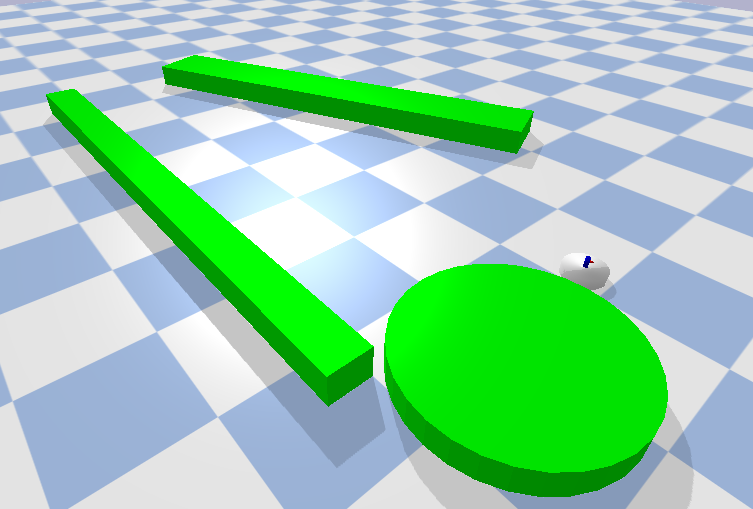
\includegraphics[width=5.0cm]{figures/example_environment_cropped.png}}; 

   \node [below, xshift=0.2cm, yshift=-.1cm, text width=5cm, align=left, outer sep=0cm] at (environment.north) {\textbf{Robot Environement}};
   
    \draw [myEvenLighterColor,
    rounded corners=0.3cm, 
    line width=0.3cm]  
    (environment.north west) -- 
    (environment.north east) --
    (environment.south east) --
    (environment.south west) -- cycle  ;
    
    \node [block,
    above of=environment,
    minimum height=2cm,
    minimum width=5cm,
    node distance=4.3cm,
    outer sep=0cm] (hgraph) {Hypothesis Algorithm};
   
    \node [block, 
    above of=hgraph, 
    node distance=3.5cm, 
    minimum width=5cm,
    minimum height=2.0cm] (kgraph) {Knowledge Graph};
      
    \node [rectangle, draw, 
    fill=myEvenLighterColor, 
    text width=5em, text centered, rounded corners, 
    right of=kgraph, 
    minimum width=4cm,
    minimum height=2cm,
    node distance=8cm] (ontology) {Ontology};
     
    \node [rectangle, draw, 
    fill=myEvenLighterColor, 
    text width=5em, text centered, rounded corners, 
    right of=hgraph, 
    minimum width=4cm,
    minimum height=2cm,
    node distance=8cm] (planner) {High-level planner};
    
    % Draw edges
    \draw[-stealth] ([yshift=0.155cm, xshift=0.4 cm]environment.north) -- node [right] {\shortstack[]{sensor\\measurements}}([xshift=0.4 cm]hgraph.south) ;
    \draw[-stealth] ([xshift=-0.4 cm]hgraph.south) -- node [left] {robot input}([yshift=0.155cm, xshift=-0.4 cm]environment.north) ;
    \draw[-stealth] (planner.west) -- node [pos=0.37, above] {task}(hgraph.east);
    \draw[-stealth] ([xshift=-0.4cm]kgraph.south) -- node [left] {\shortstack[]{action\\suggestions}}([xshift= -0.4cm]hgraph.north) ;
    \draw[stealth-] ([xshift=0.4cm]kgraph.south) -- node [right] {action feedback}([xshift= 0.4cm]hgraph.north) ;
    \draw[-stealth] (kgraph.east) -- node [above, pos=0.63] {\shortstack[]{environment\\knowledge}}(ontology.west);
    \draw[stealth-] ([xshift=0.4cm]ontology.south) -- node [right] {\shortstack[]{query}}([xshift=0.4cm]planner.north);
    \draw[-stealth] ([xshift=-0.4cm]ontology.south) -- node [left] {\shortstack[]{output}}([xshift=-0.4cm]planner.north);
    \draw[stealth-] (planner.south) |- ++ (2,-1) node[near end, above] {\shortstack[]{High-level\\task}};
    \end{tikzpicture}
\caption{Simplified flowchart representation of the proposed method.}
\label{tikz:flowchart_proposed_method}
\end{figure}
\todo[inline]{Review/restyle/update the flowchart here above}


\subsection{Definition}%
\label{subsec:hgraph_definition}%
Before defining the \ac{hgraph}, some definitions are defined on which the \ac{hgraph} depends. First, recall the \textbf{state} defined in the \cref{sec:problem_description}.\bs

An object holds the information about an object.\\Formally, a \textbf{object},  $obst_{id}(k) = \left\langle s(k), shape \right\rangle $\bs

where $shape$ is linked to a 3D representation of the object which is used to construct the configuration space.\bs

An object node represents an object in a state.\\Formally, a \textbf{objectNode}, $V^{obst}_{id} =\left\langle \textrm{status}, obst(k)\right\rangle $\\where status indicates if the node has been visited in the \ac{hgraph}. $\textrm{status} = (Initialised, Completed, Failed)$\bs

An edge describes the details of how a node transitions to another node in the \ac{hgraph}. In the robot environment, an edge represents a change of state for an object. System identification and performing an action such as pushing or driving both change the state of objects in the robot environment, but because are very different, the edges are split into 2 categories. IdentificationEdges that collect system \ac{IO} data and convert that into a system model. And actionEdges that plan and track a motion from a start to a target state. Formally:\bs

A \textbf{identificationEdge},
\todo[inline]{define identificationEdge, currently hard coded models are used in the implementation}

A \textbf{actionEdge}, $\tau_{(from, to)} = \left\langle \textrm{status}, id_{from}, id_{to}, \textrm{verb}, \textrm{controller},\textrm{dynamic model}, \textrm{path}\right\rangle$\bs

with $id_{from}$ and $id_{to}$ indicating the node id of the node in the \ac{hgraph} where the edge start from and point to respectively, $verb$ an English verb describing the action the edge represents, the controller contains the controller used for driving the robot, the dynamic model is the dynamic model used by the controller, path a list of configurations indicating the path connecting a start- to target node.\bs
\todo[inline]{Martijn: what does this mean: "the controller contains the controller..."?}

A $verb = \{\textrm{driving, pushing}\}$.\bs

Now the nodes and edges have been defined, the \ac{hgraph} can be defined.\bs

Formally, a \textbf{hypothesis graph}, $G^{hypothesis} = \left\langle V, E \right\rangle $ 
\\comprising $V = \{V^{ob}_{i}\}$, \quad $E \in \{\tau_{(i,j)}| V_i, V_j \in \{V^{ob} \}, i \neq j\}$.\bs

Most \ac{hgraph} components have now been defined. The status of an identification edge or action edge still remains undefined and requires some further explanation.\bs

\paragraph{Status, Types and Lifetime of edges}
Because system identification and tracking a path are so very different, the edges are split into two categories, identification edges and action edges. An identification edge, which is responsible for sending an input sequence to the system and recording the system output. That input/output sequence and assumptions on the system are the basis for system identification, techniques on various system identification methods are discussed in \cref{sec:sys_iden}. The goal is to create a dynamical model which is augmented with a corresponding controller is closed-loop stable.\bs

An identificationEdge, the status can be visualised in \cref{tikz:status_identification_edge}.\bs

\begin{figure}[H]
\centering
\begin{tikzpicture}[node distance = 2cm, auto, initial]
    \node [state, fill=my_dark_blue] (init_test_num) {IT\#t};
    \node [state, fill=my_light_blue, below of=init_test_num] (completed_test_num) {CT\#t};
    \node [state, accepting, fill=my_green, below of=completed_test_num] (completed) {CO};
    \node [state, accepting, fill=my_red, right of=completed_test_num, node distance=6cm] (failed) {FAIL};

 % arrows
    \draw [-stealth] ([xshift=-2cm]init_test_num.west) to node[near start,above]{\shortstack[]{select compatible\\sys. iden. method}} (init_test_num.west);
    \draw[-stealth] (init_test_num) edge[bend right] node[left]{Collect \ac{IO} data} (completed_test_num)
(completed_test_num) edge node[left]{create system model} (completed);
    \draw [-stealth] (completed_test_num) edge[bend right] node[right]{goto next start state} (init_test_num);
    \draw [-stealth] (completed_test_num) to node[]{Unable to reach next start state}  (failed.west);
    \draw [-stealth] (init_test_num) [out=0, in=90] to node[above]{Unable to reach next pos}  (failed.north);

\end{tikzpicture}
\caption{\acs{FSM} displaying the status of an identification edge}%
\label{tikz:status_identification_edge}
\end{figure}

\todo[inline]{some explainer on this status of iden edge}

The second type of edge is an actionEdge, containing a drive or push action. An actionEdge ready for execution contains all the necessary information to send input to the robot resulting in an object being steered toward it's target state. Before an edge is ready for execution it should be initialised properly, more specifically: initialised, path estimated should be performed, a system model must be initiated and path planning must be performed. Then finally the edge is ready to be executed and send input toward the robot, an \ac{FSM} of the actionEdge's status can be visualised in \cref{tikz:status_action_edge}.\bs

\begin{figure}[H]
\centering
\begin{tikzpicture}[node distance = 2cm, auto, initial]
    % \node [state, fill=lavenderIndigo] (init) {IN};
    \node [state, fill=my_purple] (init) {IN};
    \node [state, fill=my_dark_blue, below of=init] (path_exist) {PE};
    \node [state, fill=my_light_blue, below of=path_exist] (system_model) {SM};
    \node [state, fill=my_green, below of=system_model] (path_planned) {PP};
    \node [state, fill=my_yellow, below of=path_planned] (executing) {EX};
    \node [state, accepting, fill=my_orange, below of=executing] (completed) {CO};
    \node [state, accepting, fill=my_red] (failed) at ([xshift=4cm]$(system_model)!0.5!(path_planned)$) {FAIL};
    
 % arrows
    \draw [-stealth] ([xshift=-2cm]init.west) to node[near start,above]{select controller} (init.west);
    \draw[-stealth] (init) edge node[left]{graph-based path estimation} (path_exist)
      (path_exist) edge[bend right] node[left]{load in system model} (system_model)
(system_model) edge[bend right] node[left]{motion planning} (path_planned)
(path_planned) edge[bend right] node[left]{goto execution loop} (executing)
(executing) edge[bend right] node[left]{completed} (completed);

    \draw [-stealth] (init.east) [out=0, in=90] to node[xshift=0.1cm, right]{path non-existence proven}  ([yshift=-0.03cm,xshift=0.2cm]failed.north);
    \draw [-stealth] (path_exist.east) [out=0, in=90] to node[xshift=-0.6cm,yshift=0.55cm, above]{\shortstack[l]{system\\identification\\error}}  ([yshift=-0.03cm,xshift=-0.2cm]failed.north);
    \draw [-stealth] (system_model.east) [out=0, in=180] to node[xshift=0.1cm, yshift=0.3cm, above]{\shortstack[l]{motion\\planning\\error}} (failed.west);
    node[right]{motion planning error}  
    ([yshift=-0.3cm]failed.west);
    \draw [-stealth] (executing.east) [out=0, in=-90] to node[xshift=0.1cm,right]{fault detected}(failed.south);

\end{tikzpicture}
\caption{\acs{FSM} displaying the state of an action edge}%
\label{tikz:status_action_edge}
\end{figure}

% \par\smallskip\noindent
\centerline{\begin{minipage}{0.8\textwidth}
\begin{enumerate}
  \item[INITIALISED (IN)] The edge is created with a source and target node which are present in the \ac{hgraph}. A choice of controller is made.
    \item[PATH EXISTS (PE)] A graph-based search is performed to validate if the target state is reachable assuming that the system is holonomic.
    \item[SYSTEM MODEL (SM)] A dynamics system model is provided to the controller residing in the edge.
    \item[PATH PLANNED (PP)] Resulting from a sample-based planner, a path from start to target state is provided. 
    \item[EXECUTING (EX)] The edge is currently receiving observations from the robot environment and sends back robot input. 
    \item[COMPLETED (COMPL)] The edge has driven the system toward its target state and its performance has been calculated.
    \item[FAILED (FAIL)] An error occurred, yielding the edge unusable. 
\end{enumerate}
\end{minipage}}
\par\smallskip

\Cref{tikz:status_action_edge} shows that many steps must successfully be completed before the robot can start executing. The performance of an edge during execution, measured in various metrics (\cref{sec:proposed_method_metrics} is dedicated to metrics) is dependent on many aspects. Such as the choice of controller, the path estimation, the system model yielded by the identification edge and the path yielded by motion planning. Now that he \ac{hgraph} is defined, let's see how it is generated in the upcoming section.\bs


\subsection{System Identification and Control Methods}
\label{subsec:sys_iden_and_control_methods}

\subsection{Estimating Path Existence}%
\label{subsec:estimating_path_existence}

Graph-based planning

\quotes{The main idea is to discretise the configuration space with a finite discretisation. The emerged cells act as nodes in the graph, cells are connected through edges to nearby cells. Graph-based planners start from the cell containing the starting pose and search for the cell containing the target pose whills avoiding cells which lie in obstacle space.}
\todo[inline]{check de quote hierboven}



\subsection{Motion Planning}%
\label{subsec:motion_planning}

Controllers discussed in \cref{subsec:sys_iden_and_control_methods} can track a path from start to target. Providing a path is a the motion planners responsibility, motion planners seek inside the configuration space for a path from start to target configuration. A practical example of such an path is a list of successive robot poses, from starting pose (coinciding with the starting configuration) toward the target pose, where the successive poses lie close together (reachable for the robot in $\sim20$ time samples). Seeking a path from start to target inside a configuration space whilst avoiding obstacles for the robot to track is referred to as \textit{motion planning}. Finding a path between start and target configuration for pushing application avoiding collision is referred to as \textit{manipulation planning}. First this subsection presents motion planning, next subsection, \cref{subsec:manipulation_planning} dedicates itself to manipulation planning. For both motion and manipulation planning sampling based methods are used, that can be discribed as.\bs

\textit{\quotes{The main idea is to avoid the explicit construction of the object space, and instead conduct a search that probes the configuration space with a sampling scheme. This probing is enabled by a collision detection module, which the motion planning algorithm considers as a “black box.”~\cite{lavalle_planning_2006}}}\bs

Generally the configuration space motion planners plan in consists of 2 subspaces, free and obstacle space. The configuration space in this thesis consists of 4 subspaces, namely free, obstacle, unknown and movable space. To solve motion planning problems for such a configuration space a dedicated motion planning algorithm has been developed that extends the existing algorithm extends the existing double tree \ac{RRT*} algorithm~\cite{chen_fast_2018}. The motion planner consists of.
\begin{center}
\begin{tabular}[t]{l p{10cm}}
$V$:& A set of nodes\\
$E$:& A set of edges\\
$P$:& A set of paths\\
\end{tabular}
\end{center}

The start connectivity tree consists of the nodes connected by edges containing the starting node, and vise versa for the target connectivity tree containing the target node. The algorithm grows the two \textit{connectivity trees} by randomly sampling configurations and adding them to the start or target connectivity tree. The algorithm explores configuration space by growing these connectivity trees. When the start connectivity tree meets the target connectivity tree a path from start to target is found.\bs

Newly sampled configurations are added is a structural manner that guarantee an optimal path is found with infinite sampling. Where optimality is defined as the path with the lowest cost. The cost is defined as a sum of a distance metric and a fixed penalty for paths that cross unknown or movable subspaces. Incentivising the algorithm to find a path around unknown or movable obstacles over path crossing through unknown or movable obstacles.\bs

The algorithm takes in 2 arguements, first the \textit{step size}, an maximal normalised distance between connected samples in the connectivity trees. Second, the \textit{search size} an subspace around newly sampled samples, inside this subspace a parent node is saught that results in the lowest cost, rewiring of closeby nodes happens and the other connectivity tree is searched to detects a full path form start to target.\bs

Now pseudocode of the proposed algorithm is provided in \cref{pseudocode:proposed_rrt_star}, functions used are elaborated on in \cref{table:functions_for_proposed_rrt_star}. The colored sections inside \cref{pseudocode:proposed_rrt_star} correspond the the surrounding colored box around subfigures in \cref{fig:motion_planner_adding_one_sample}. The following definitions are used by the proposed algorithm.\bs

\begin{table}[H]
\centering
\begin{tabular}[t]{l p{10cm}}
$x$:& A node containing a point in configuration space\\
$x_{init}$:& Creates a start and target node\\ 
$NotReachStop$:& True if the stopping criteria is not reached\\ 
$Sample_{random}$:& Creates a random sample in free-, movable- or unknown space\\
$Nearest(x, V)$:& Returns the nearest nodes from $x$ in $V$\\
$NearestSet(x, V)$:& Returns set of nearest nodes from $x$ in $V$\\
$Project(x, x')$:& Project $x$ toward $x'$\\
$CollisionCheck(x)$:& Returns true if $x$ is in free-, movable- or unknown space\\
$ObjectCost(x', x)$:& Returns a fixed additional cost if $x$ enters movable- or unknown space from $x'$, otherwis returns 0\\
$Distance(x, x')$:& Returns the distance between sample $x$ and $x'$\\
$CostToInit(x)$:& Find the total cost from $x$ to the initial node\\
$LocalPlannerCheck(x, x')$:& Return true if a local planner is able to connect $x$ and $x'$, otherwise return false. A system model (see \cref{subsec:sys_iden_and_control_methods}) acts a local planner\\
$InSameTree(x, x')$:& Returns true if both $x$ and $x'$ are in the same tree, otherwise return false\\
\end{tabular}
\caption{Functions used by the \cref{pseudocode:proposed_rrt_star}}
\label{table:functions_for_proposed_rrt_star}
\end{table}

\newpage
\begin{algorithm}[H]
\caption{Pseudocode for modified $\text{RRT}^*$ algorithm taking movable objects and constraints into account}
\label{pseudocode:proposed_rrt_star}
\begin{algorithmic}[1]

\hspace{-0.9cm}\colorbox{my_grey}{\parbox{\linewidth}{%
\State $V \leftarrow x_{init}$
\While{$NotReachStop$} 

\hspace{-0.1cm}\colorbox{my_light_blue}{\parbox{\linewidth}{%
    \State $Cost_{min} \leftarrow +\infty$ \algorithmiccomment{Create, check and project a new random sample}
    \State $x_{rand} \leftarrow Sample_{random}$
    \State $x_{nearest} \leftarrow Nearest(x_{rand}, V)$
    \State $x_{temp} \leftarrow Project(x_{rand}, x_{nearest})$

    \If{$CollisionCheck(x_{temp})$}
        \State $x_{new} = x_{temp}$
        \Else
        \State $Continue$
    \EndIf
}}

\hspace{-0.1cm}\colorbox{my_yellow}{\parbox{\linewidth}{%
    \State $X_{near} \leftarrow NearestSet(x_{new}, V)$ \algorithmiccomment{Find and connect new node to parent node}
    \For{$x_{near} \in X_{near}$}
    \State $Cost_{temp} \leftarrow CostFromInit(x_{near}) + Distance(x_{near}, x_{new}) + ObjectCost(x_{near}, x_{new})$
    \If{$Cost_{temp}  < Cost_{min}$}
            \If{$LocalPlannerCheck(x_{new}, x_{near})$}
            \State $Cost_{min} \leftarrow x_{temp}$
            \State $x_{minCost} \leftarrow x_{near}$
            \EndIf
        \EndIf
    \EndFor
    \If{$Cost_{min} == \infty$}
        \State $Continue$
    \Else
        \State $V.add(x_{new})$
        \State $E.add(x_{minCost}, x_{new})$
    \EndIf
}}

\hspace{-0.1cm}\colorbox{my_green}{\parbox{\linewidth}{%
    \State $Cost_{path} \leftarrow +\infty$ \algorithmiccomment{Check if newly added node can lower cost for nearby nodes}
    \For{$x_{near} \in X_{near}$} 
      \If{$InSameTree(x_{near}, x_{new})$} 
        \State $Cost_{temp} \leftarrow CostFromInit(x_{new}) + distance(x_{new}, x_{near}) + ObjectCost(x_{new}, x_{near})$
        \If{$Cost_{temp} < CostFromInit(x_{near})$}
           \If{$LocalPlannerCheck(x_{new}, x_{near})$}
              \State $E.rewire(x_{near}, x_{new})$
           \EndIf
        \EndIf
      \Else \algorithmiccomment{Add lowest cost path to list of paths}
          \State $Cost_{temp} \leftarrow CostFromInit(x_{new}) + distance(x_{new}, x_{near}) $ \newline\hspace*{10em} $+ CostFromInit(x_{near}) + ObjectCost(x_{new}, x_{near})$
          \If{$Cost_{temp}  < Cost_{path}$}
              \If{$LocalPlannerCheck(x_{new}, x_{near})$}
                  \State $Cost_{pathMin} \leftarrow x_{temp}$
                  \State $x_{pathMin} \leftarrow x_{near}$
              \EndIf
          \EndIf
      \EndIf
      \If{$Cost_{pathMin} == \infty$}
          \State $Continue$
      \Else
          \State $P.addPath(x_{new}, x_{pathMin}, Cost_{pathMin})$
      \EndIf
    \EndFor
}}

\EndWhile
}}
\end{algorithmic}
\end{algorithm}

\newpage
Now an example is provided of the proposed algorithm that creates and adds one sample in \cref{fig:motion_planner_adding_one_sample}. After adding the newly sampled sample is added tot the start connectivity tree, a sample is rewired then the target connectivity tree is connected to the start connectivity tree. The resulting path found can be visualised in \cref{fig:motion_planner_comparison}.\bs

\begin{figure}[H]
    \centering
    \begin{subfigure}{.49\textwidth}
    \centering
    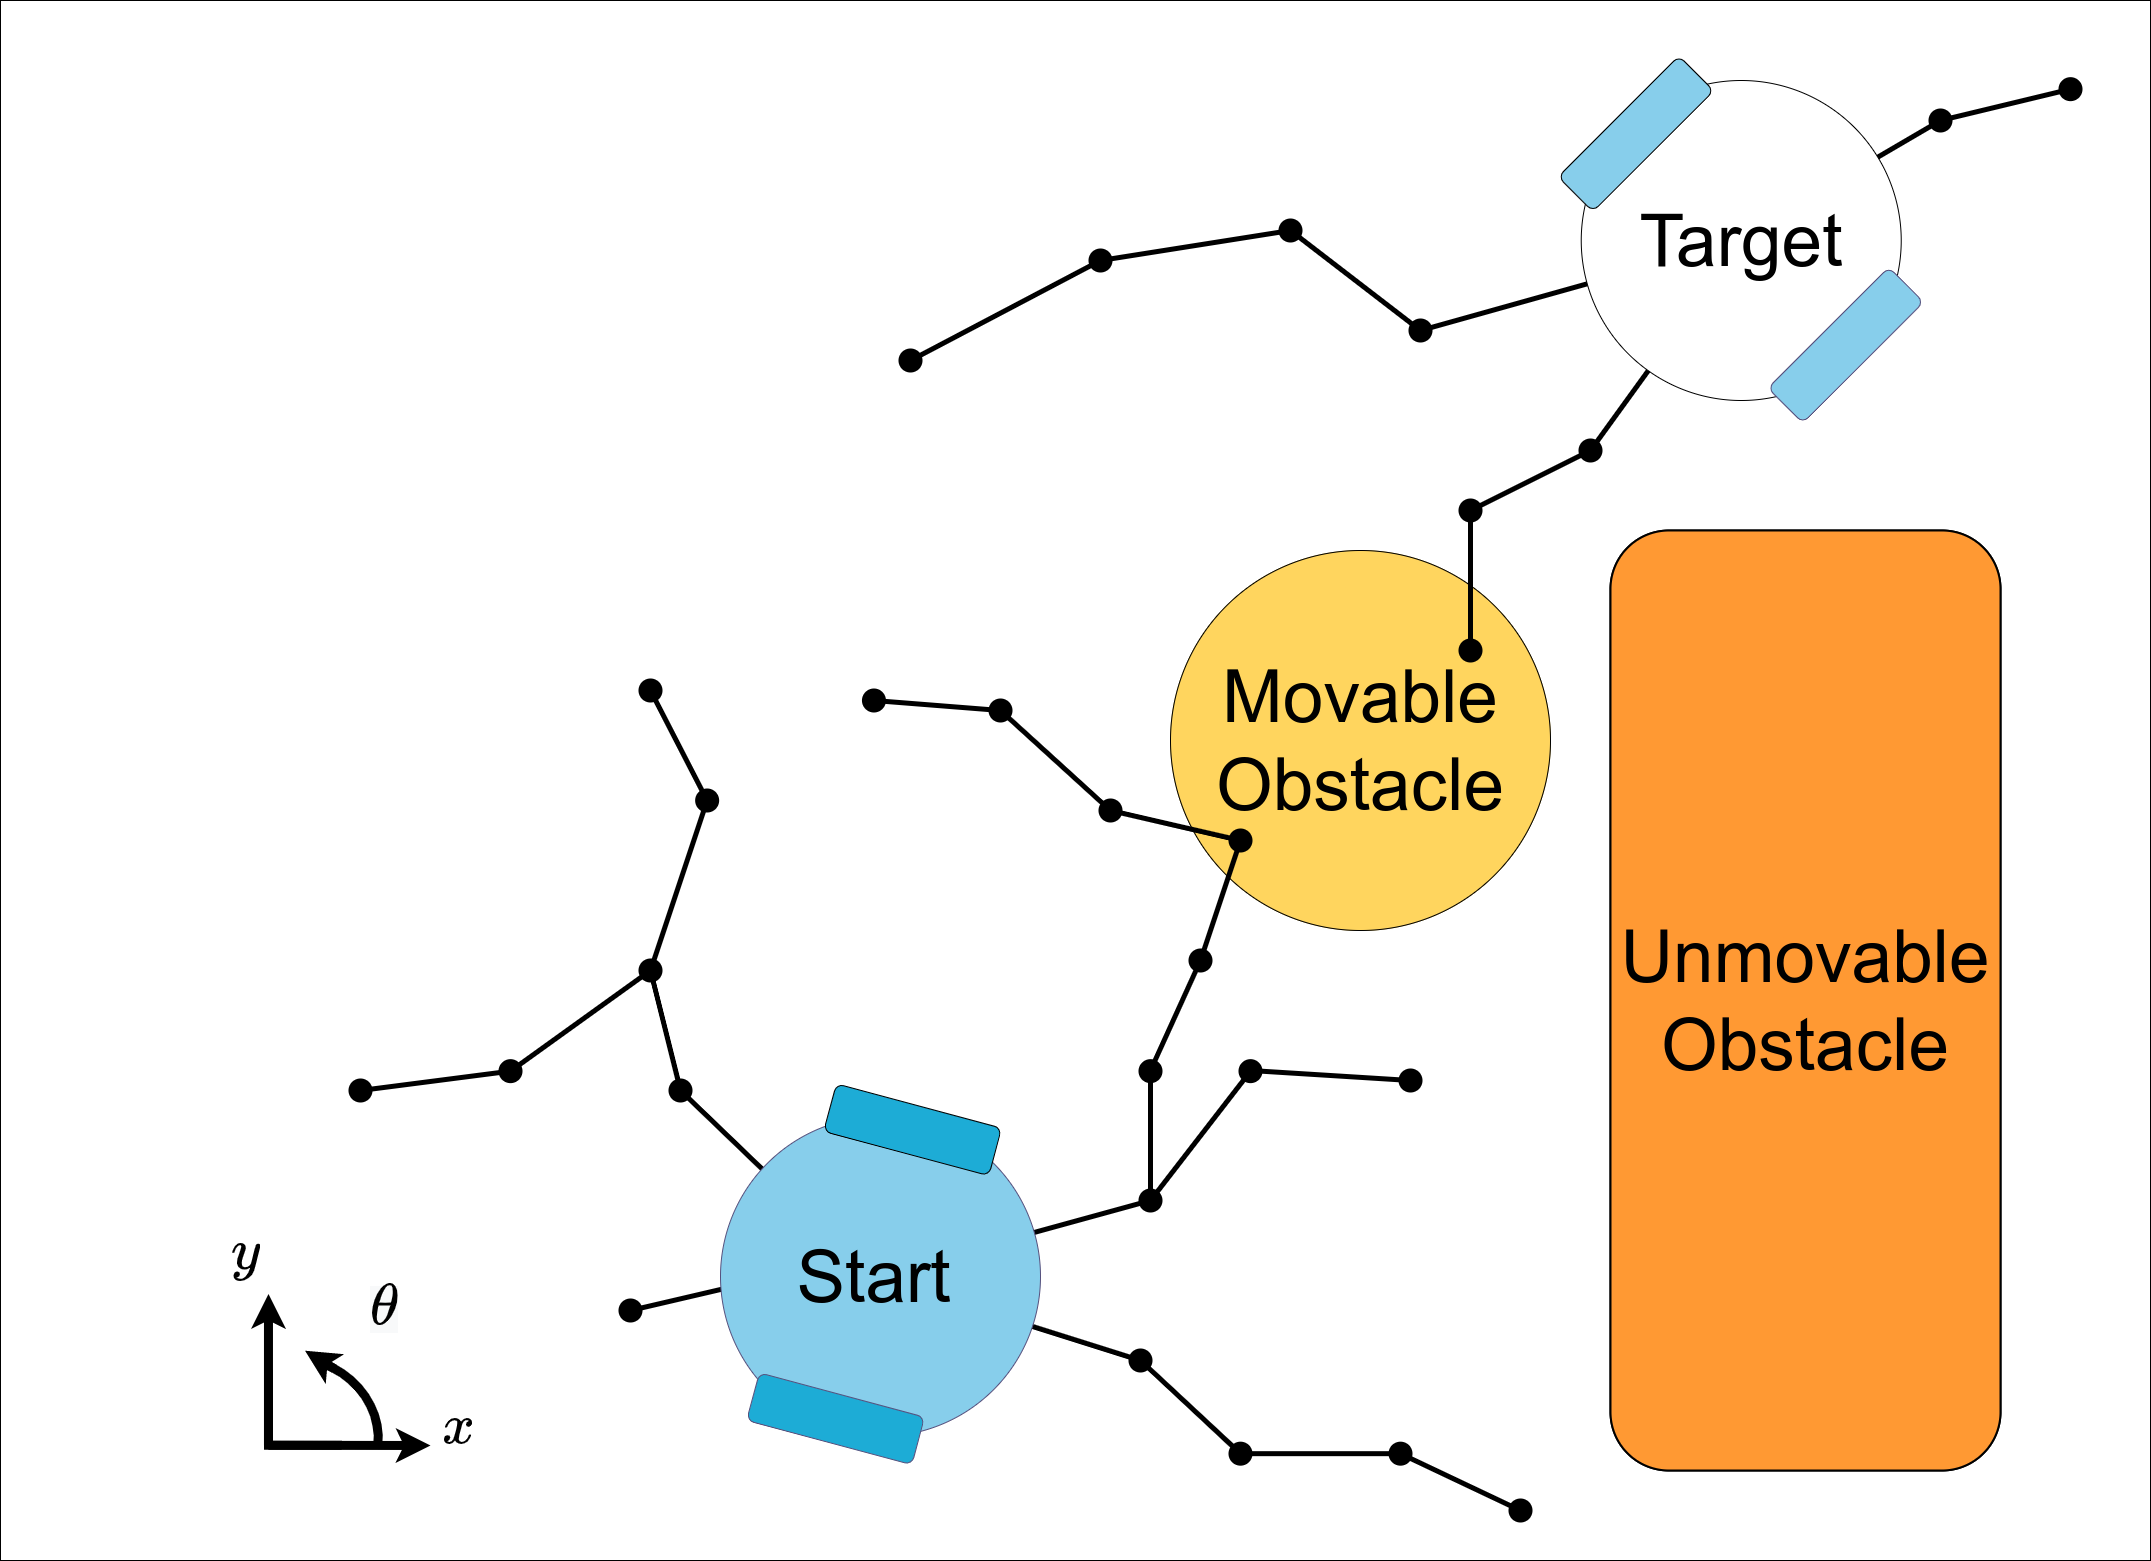
\includegraphics[width=0.93\textwidth, cfbox=my_grey 5pt 0pt]{figures/mp/1mp_init.drawio.png}
    \caption{Snapshot of the configuration space during a search\\from start to target configuration.}
    \end{subfigure}
    \begin{subfigure}{.49\textwidth}
    \centering
    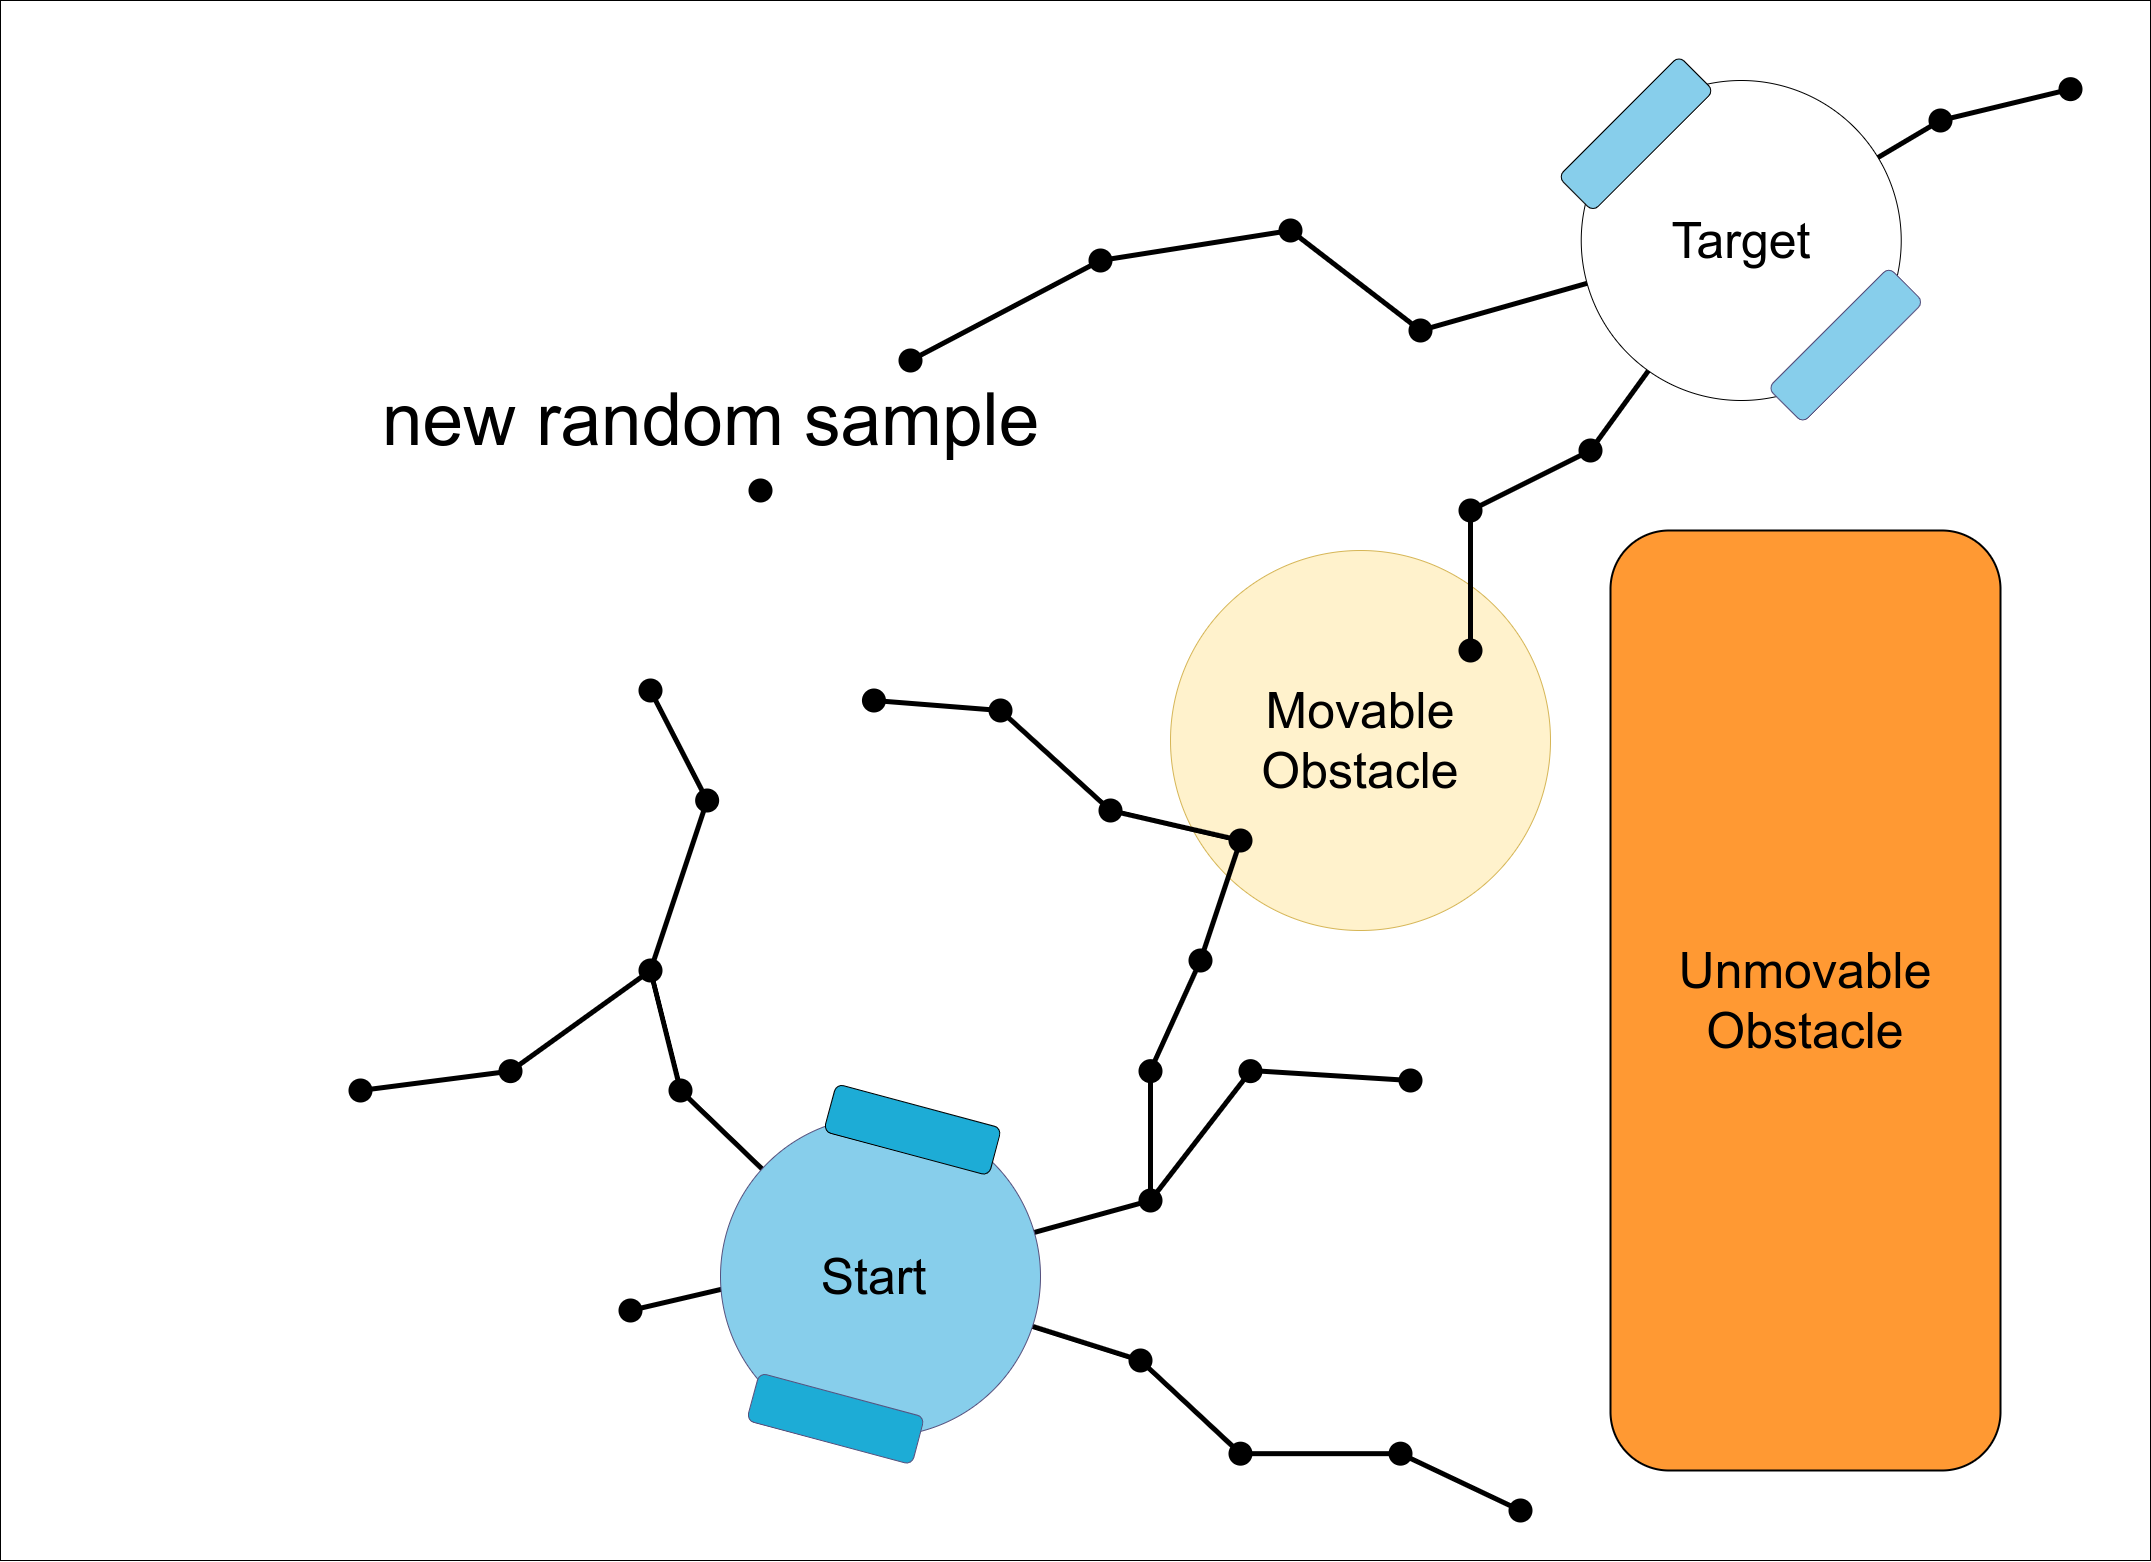
\includegraphics[width=0.93\textwidth, cfbox=my_light_blue 5pt 0pt]{figures/mp/2mp_new_rand_sample.drawio.png}
    \caption{A new random sample is generated.\bs}
    \end{subfigure}

    \begin{subfigure}{.49\textwidth}
    \centering
    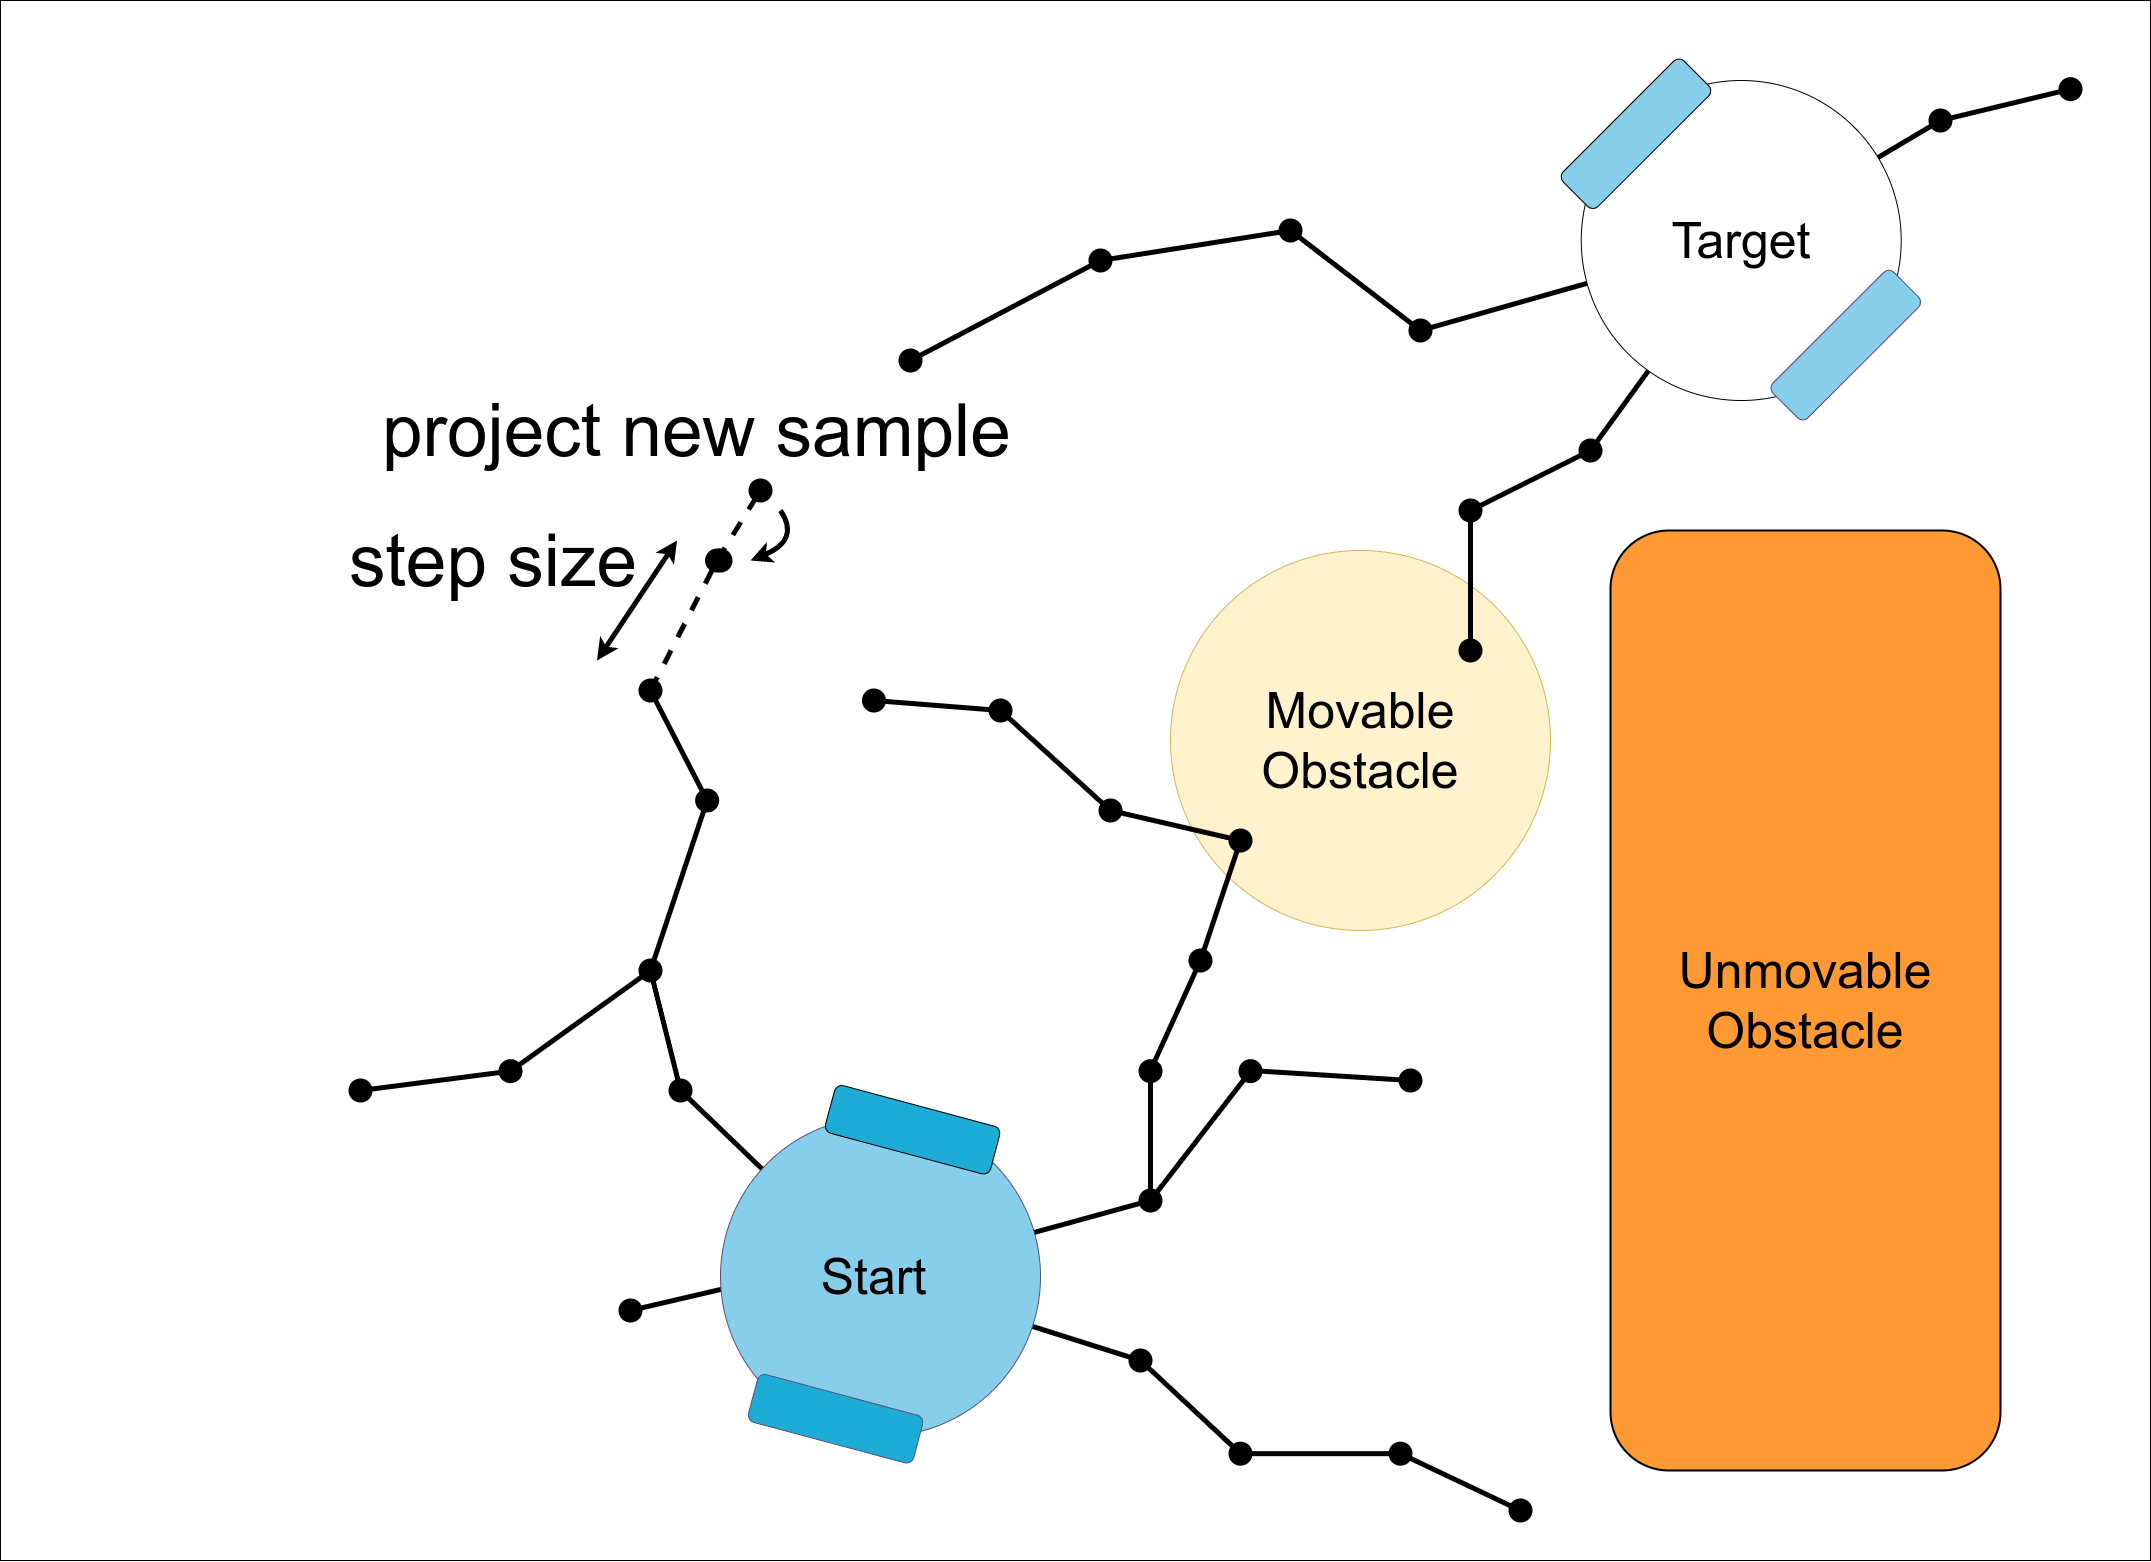
\includegraphics[width=0.93\textwidth, cfbox=my_light_blue 5pt 0pt]{figures/mp/3mp_project_sample.drawio.png}
    \caption{The new sample is projected toward the closest sample.\bs}
    \end{subfigure}
    \begin{subfigure}{.49\textwidth}
    \centering
    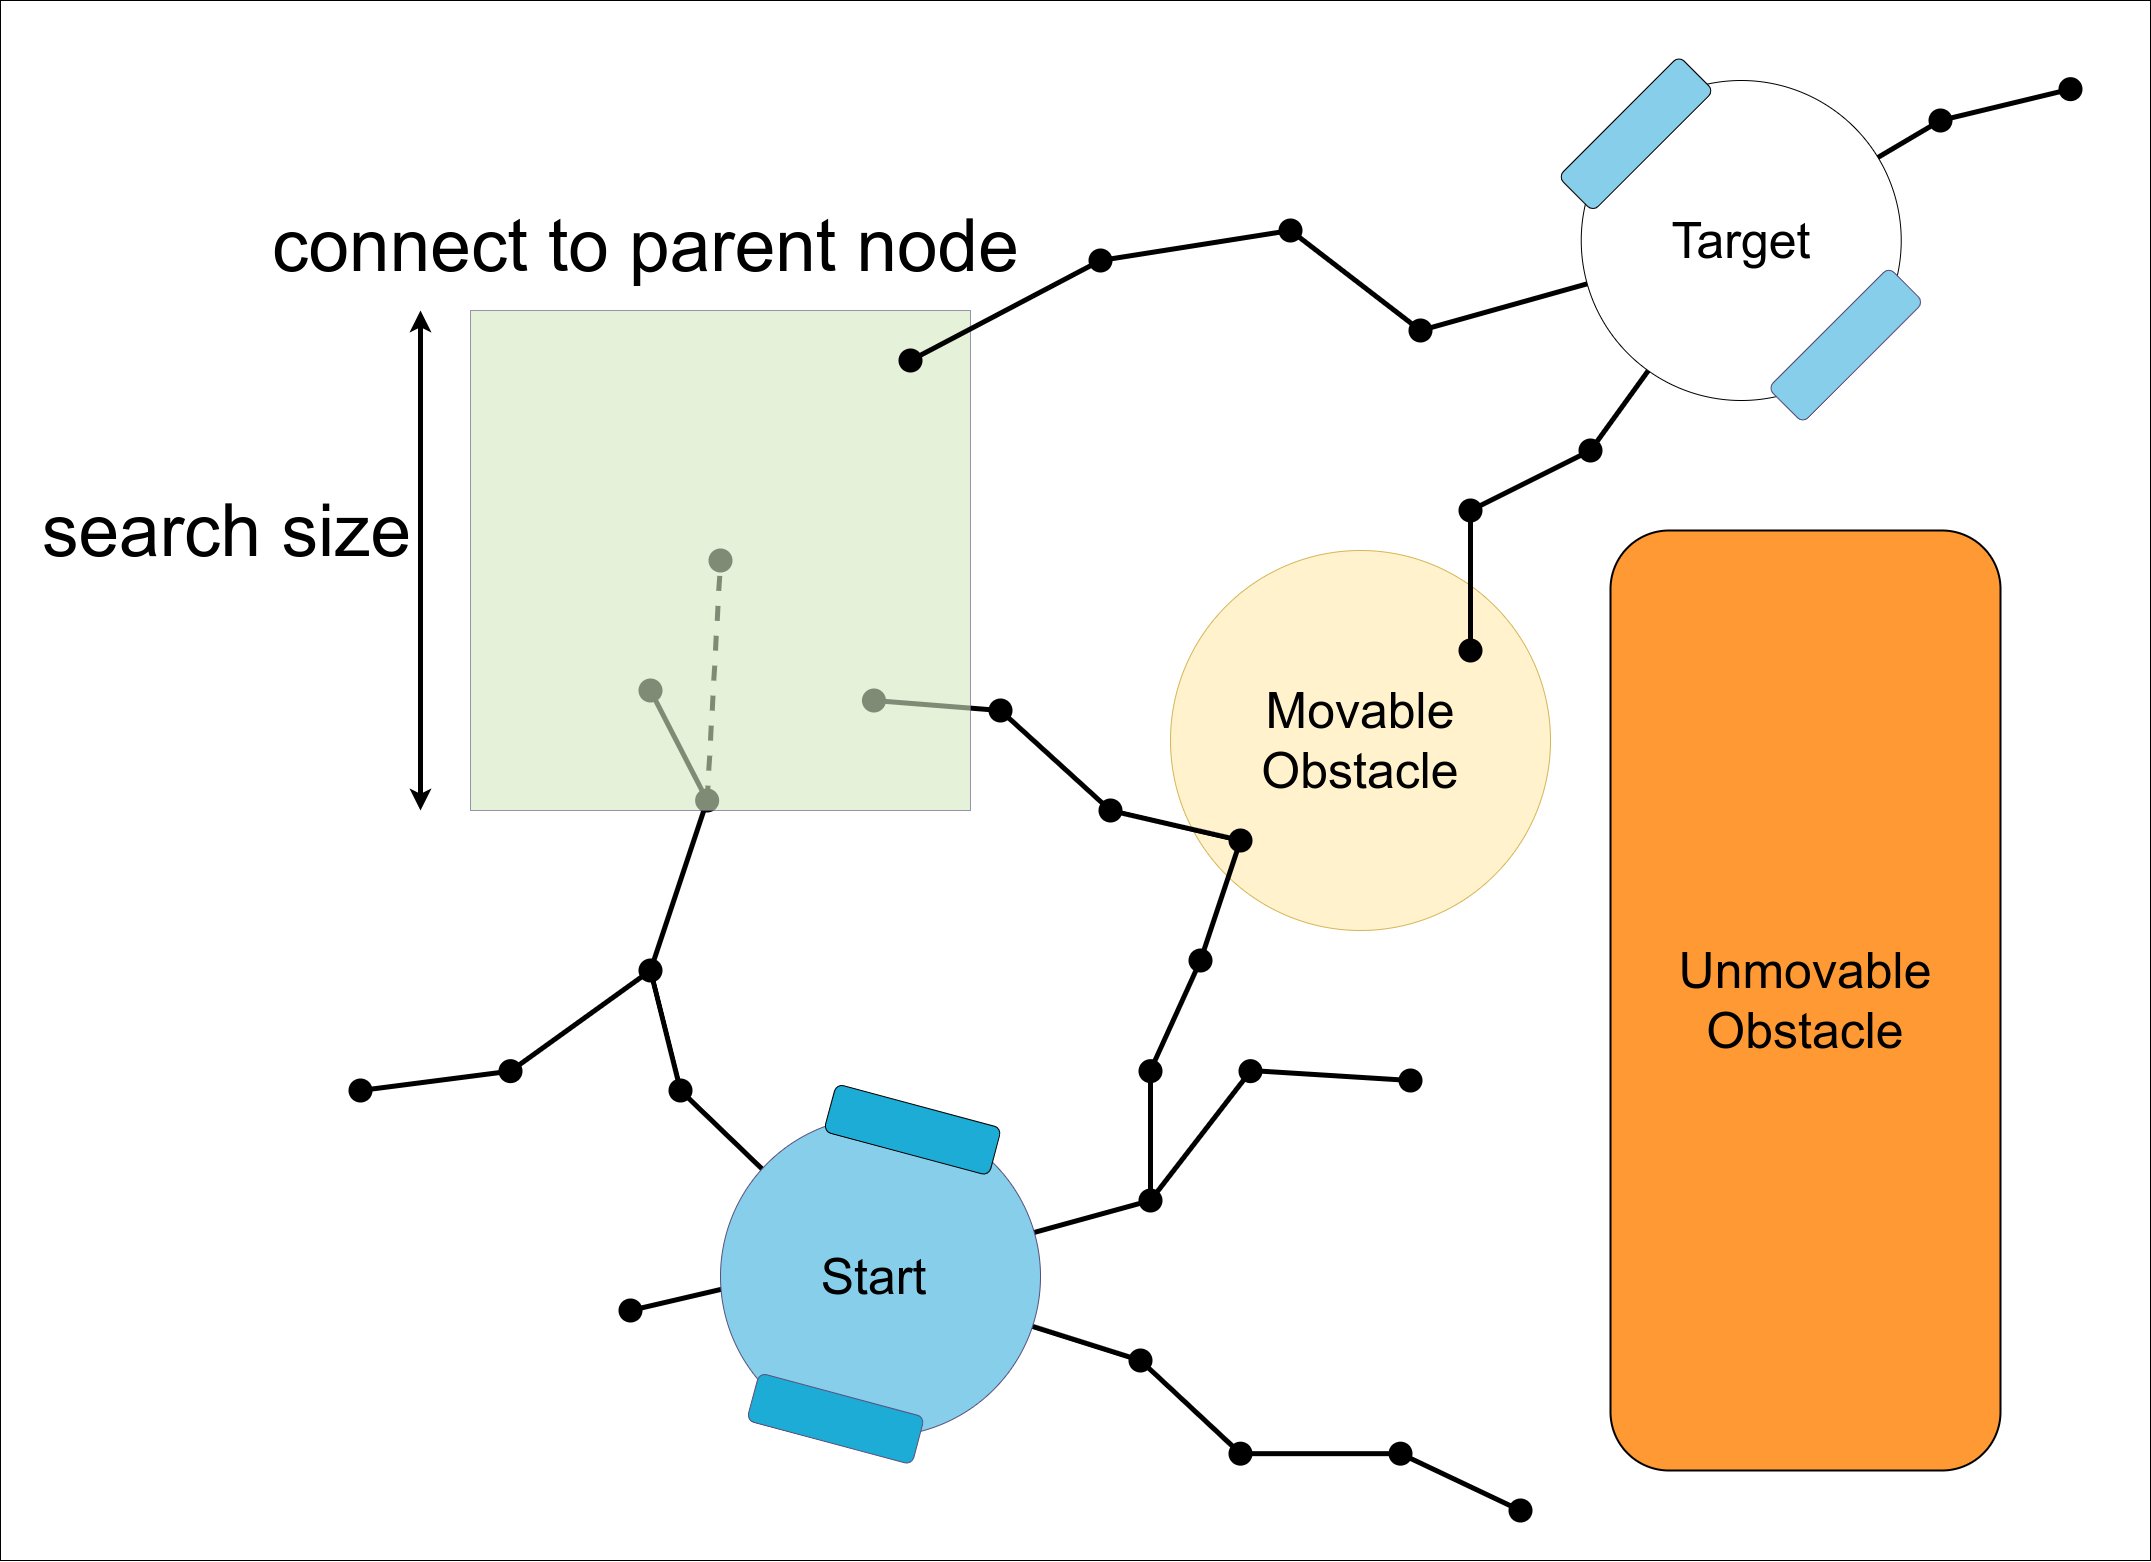
\includegraphics[width=0.93\textwidth, cfbox=my_yellow 5pt 0pt]{figures/mp/4mp_connect_to_tree.drawio.png}
    \caption{The new sample is connected to the node in search space\\that results in the lowest cost.}
    \end{subfigure}

    \begin{subfigure}{.49\textwidth}
    \centering
    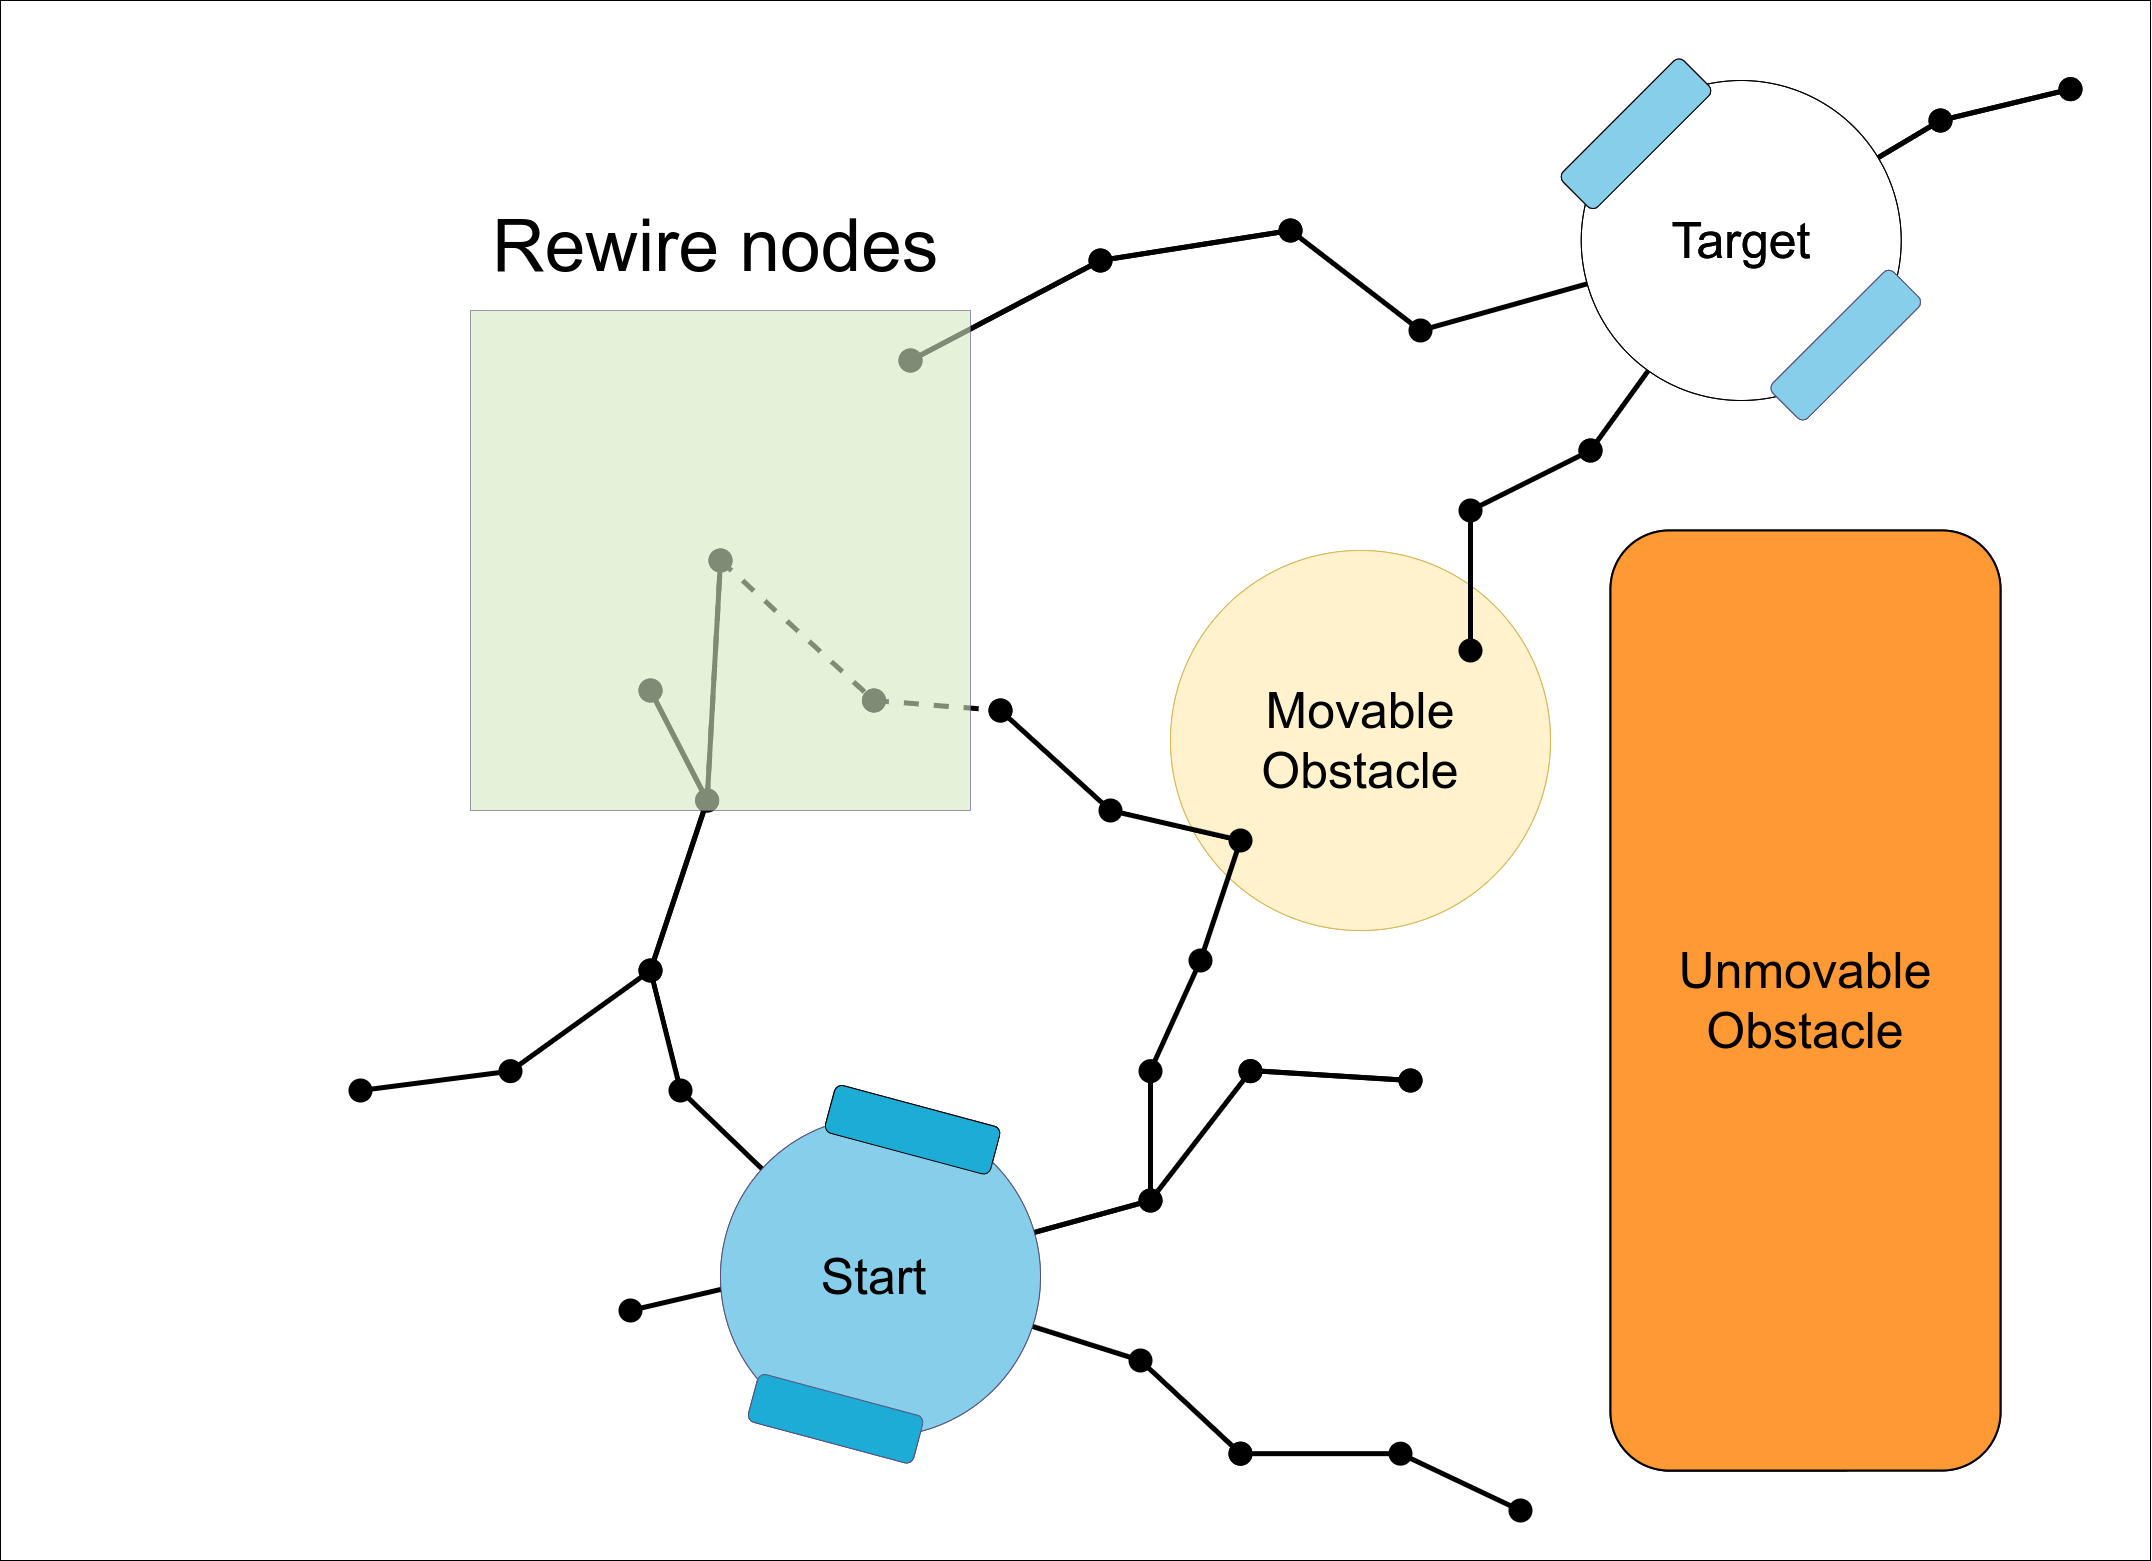
\includegraphics[width=0.93\textwidth, cfbox=my_green 5pt 0pt]{figures/mp/5mp_rewire.drawio.png}
    \caption{Nodes for which the cost can be lowered\\from the new sample are rewired.}
    \end{subfigure}
    \begin{subfigure}{.49\textwidth}
    \centering
    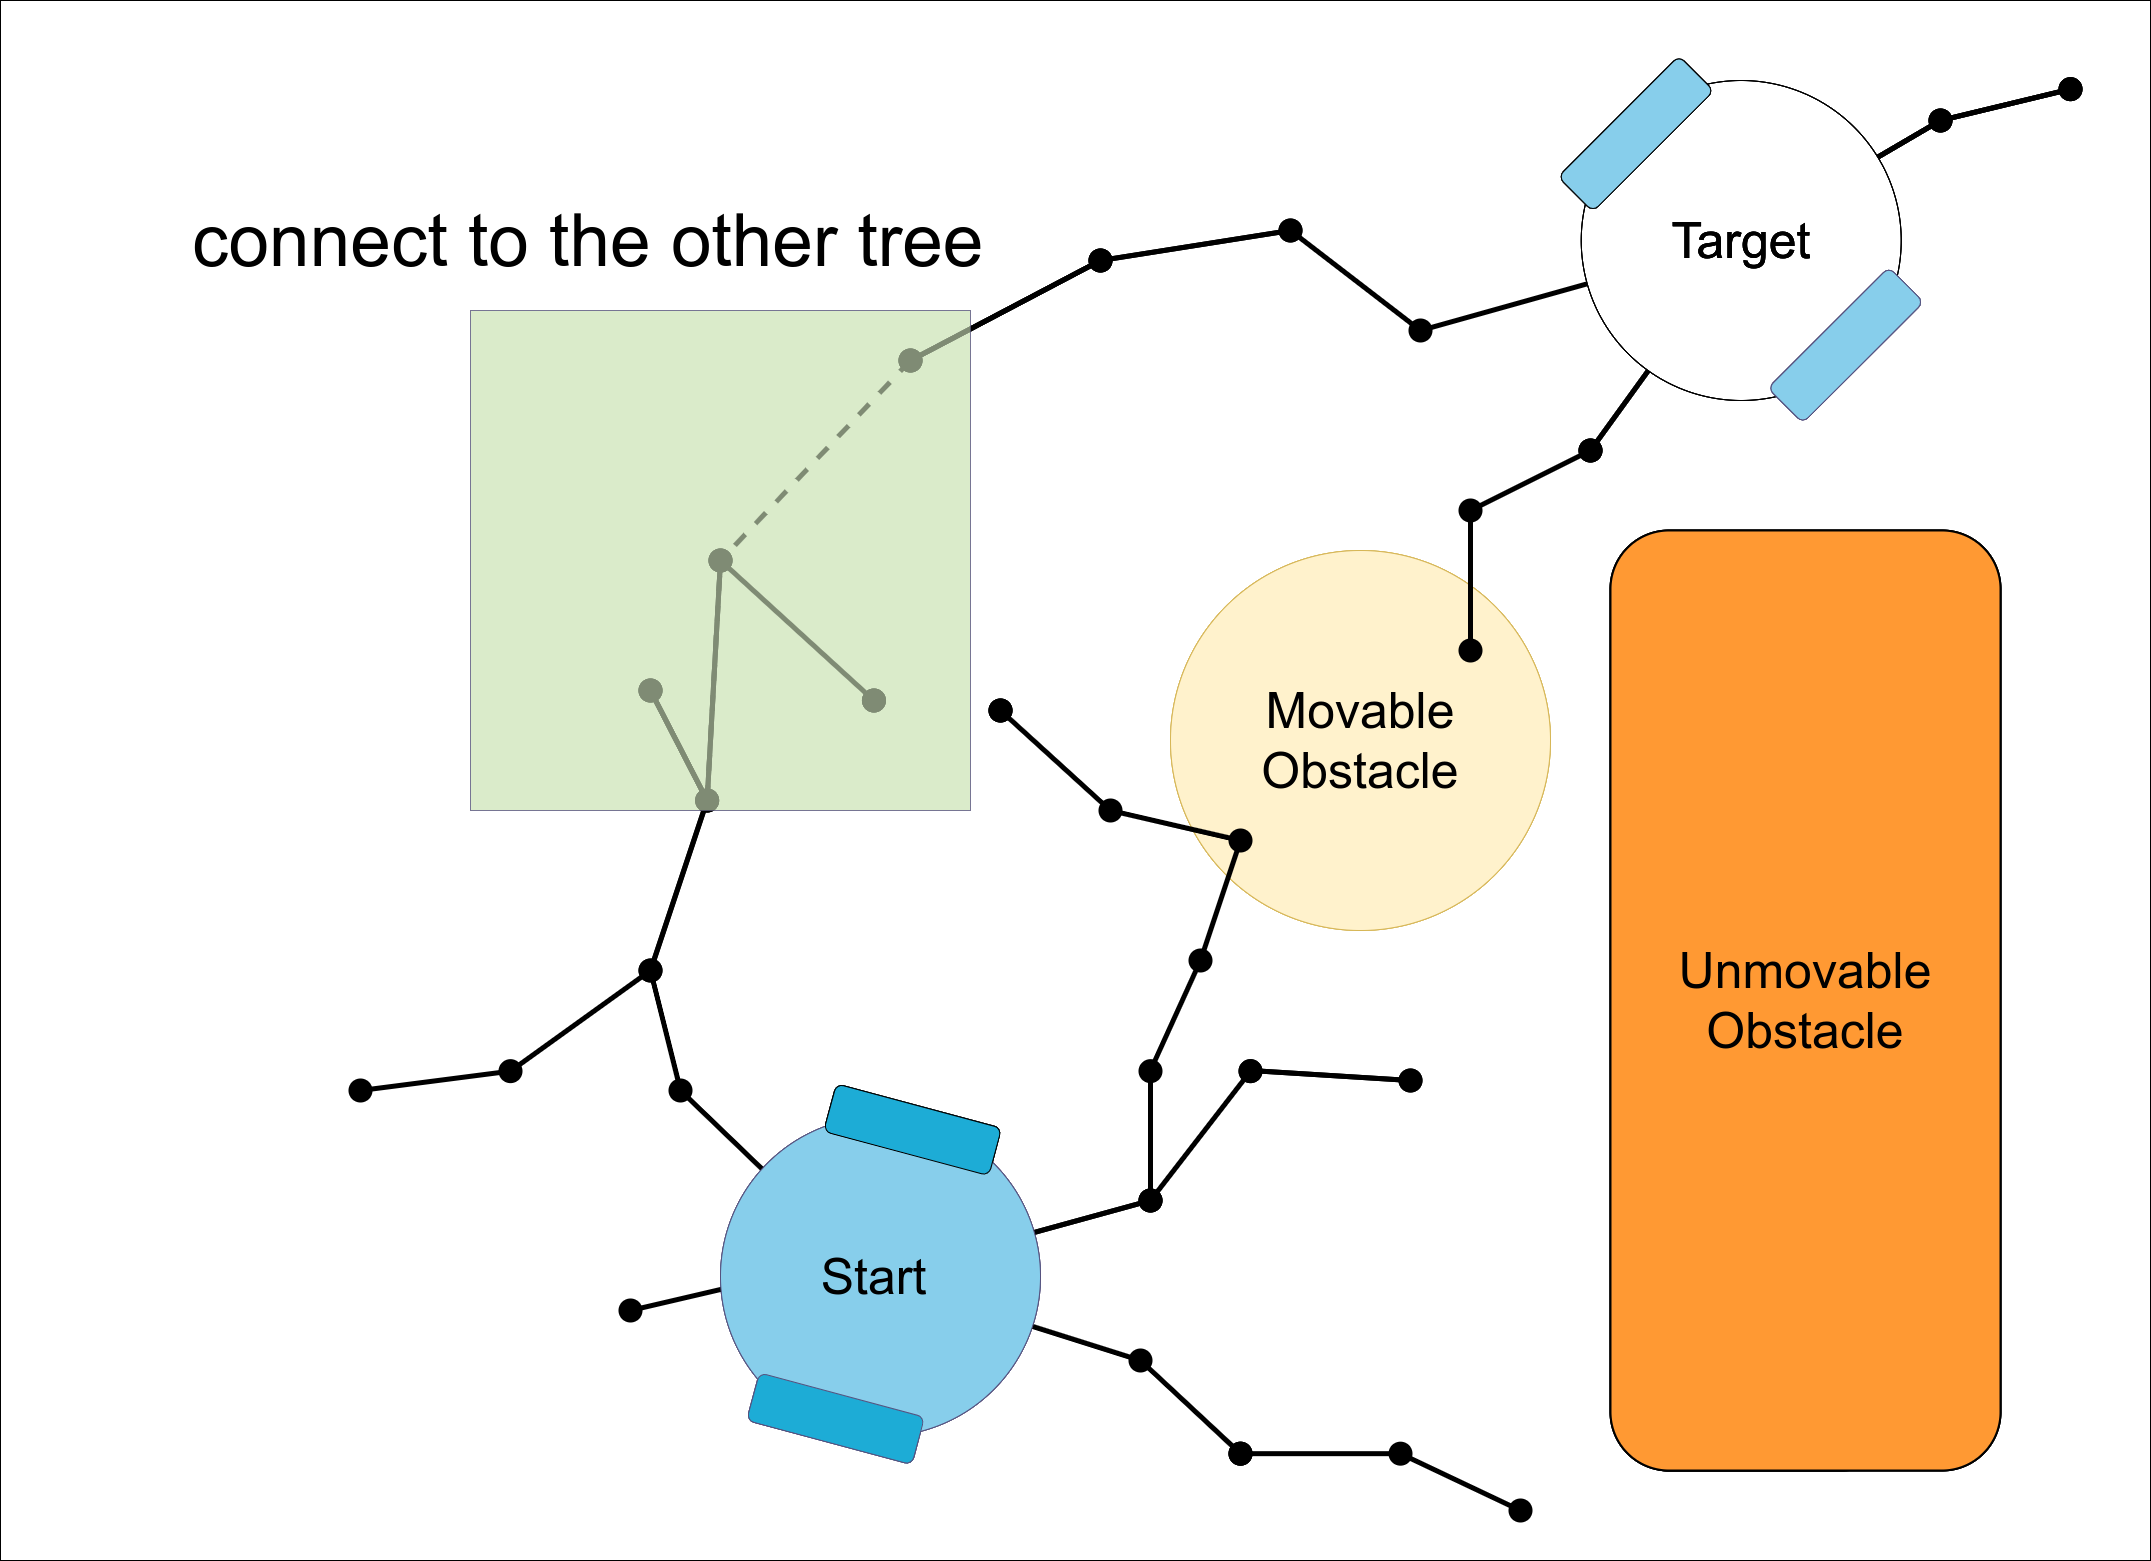
\includegraphics[width=0.93\textwidth, cfbox=my_green 5pt 0pt]{figures/mp/6mp_search_other_tree.drawio.png}
    \caption{A path from start to target configuration is found. \bs}
    \end{subfigure}

    \caption{Visualisation of the Double tree \acs{RRT*} motion planner that add a single sample to the connectivity graph. The color of the box surrounding subfigures corresponds to the colored sections in \cref{pseudocode:proposed_rrt_star}. 3 dimensional configuration space displayed as 2 dimensional configuration space ($x$ and $y$ are visable, $\theta$ is not visable).}
    \label{fig:motion_planner_adding_one_sample}
\end{figure}


\begin{figure}[H]
    \centering
    \begin{subfigure}{.5\textwidth}
    \centering
    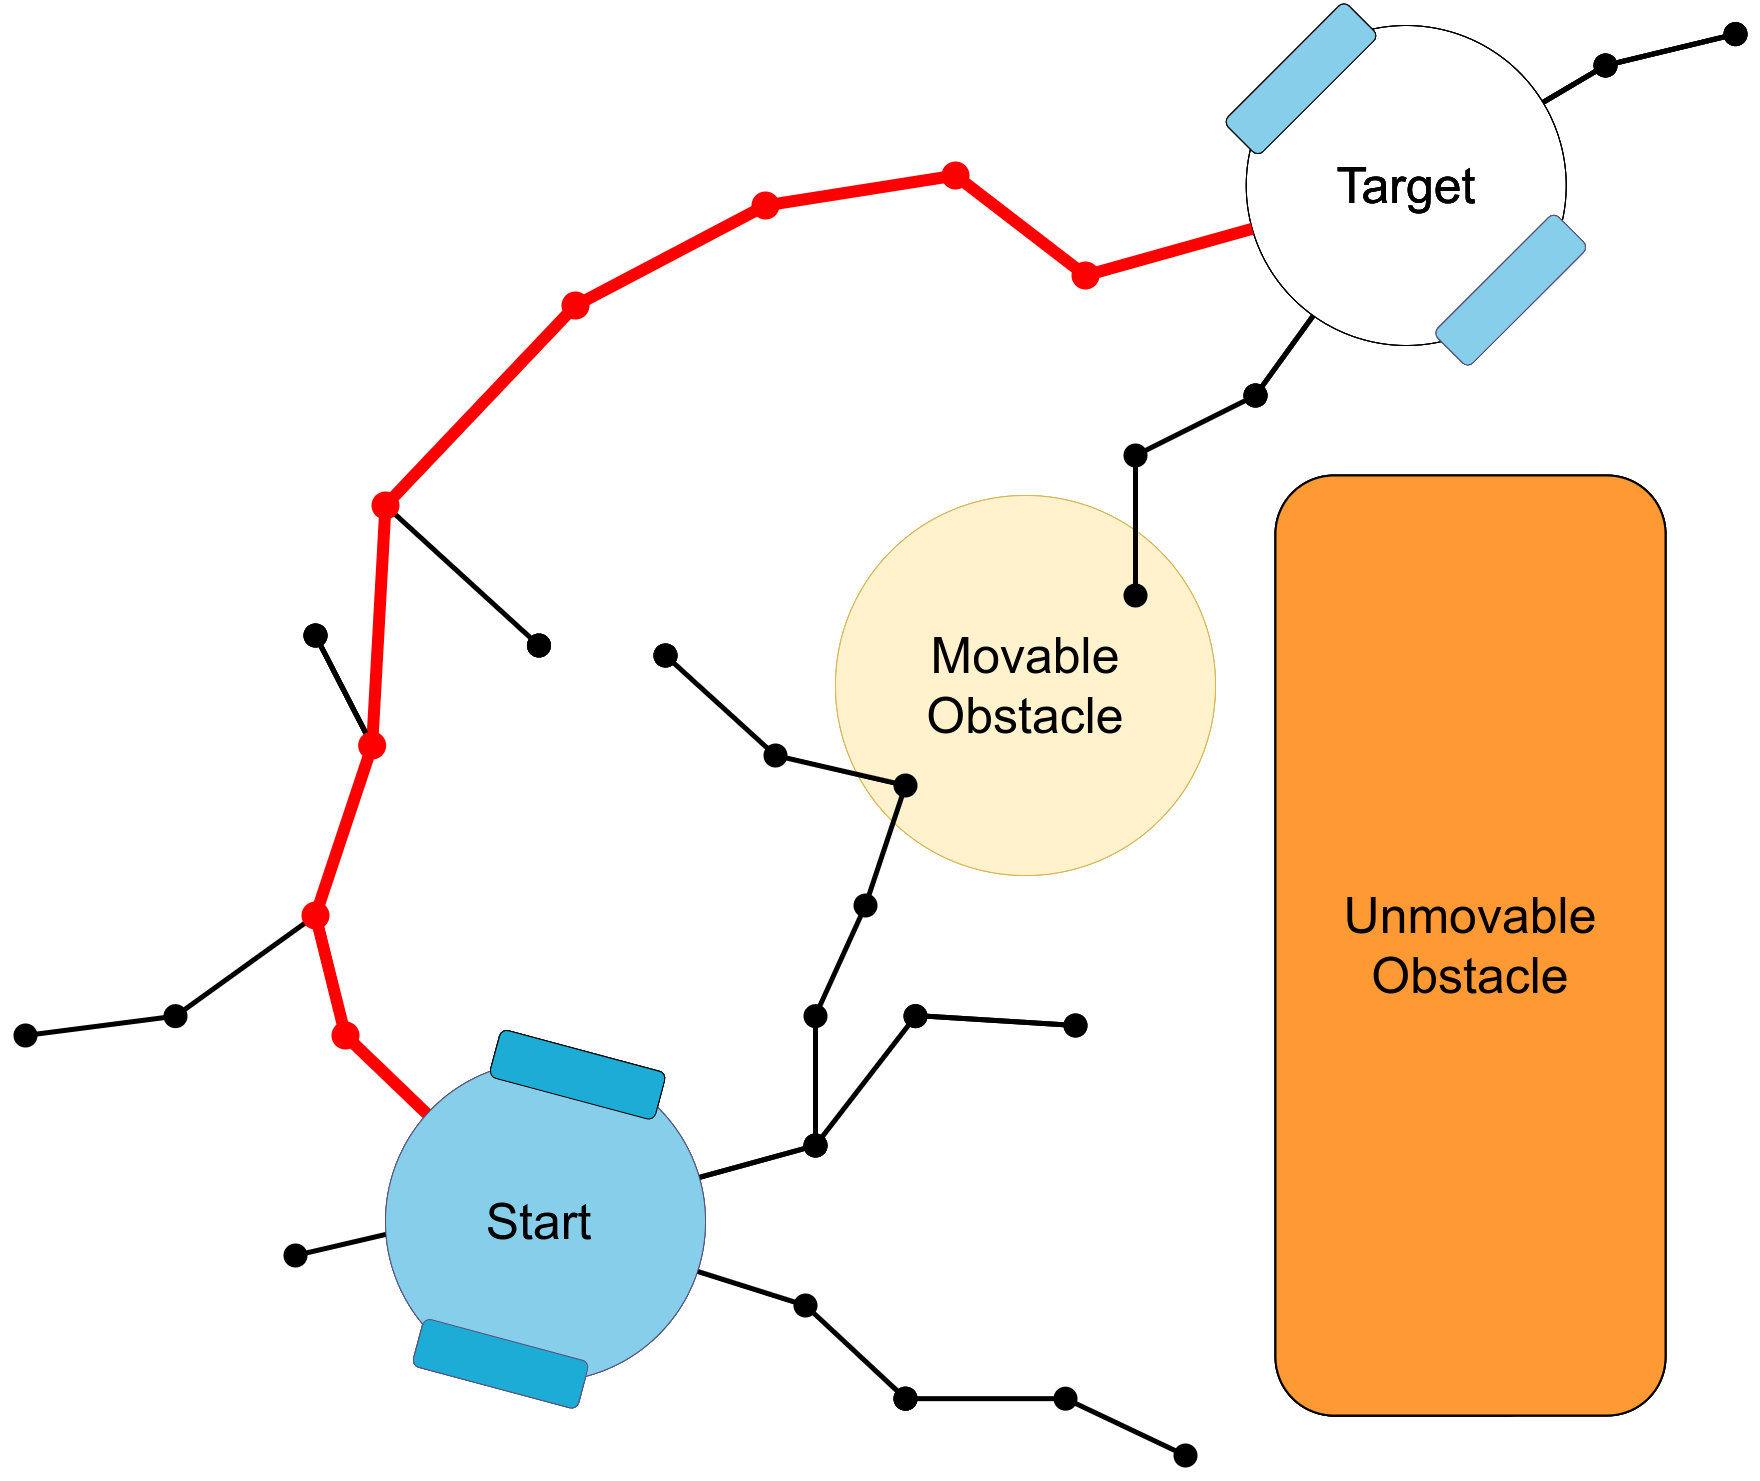
\includegraphics[width=0.8\textwidth]{figures/mp/7mp_path_found.drawio.png}
    \caption{The resulting configuration space after sample in \cref{fig:motion_planner_adding_one_sample}\\ was added. The path found is marked in red}
    \end{subfigure}%
    \begin{subfigure}{.5\textwidth}
    \hspace{-1cm}
    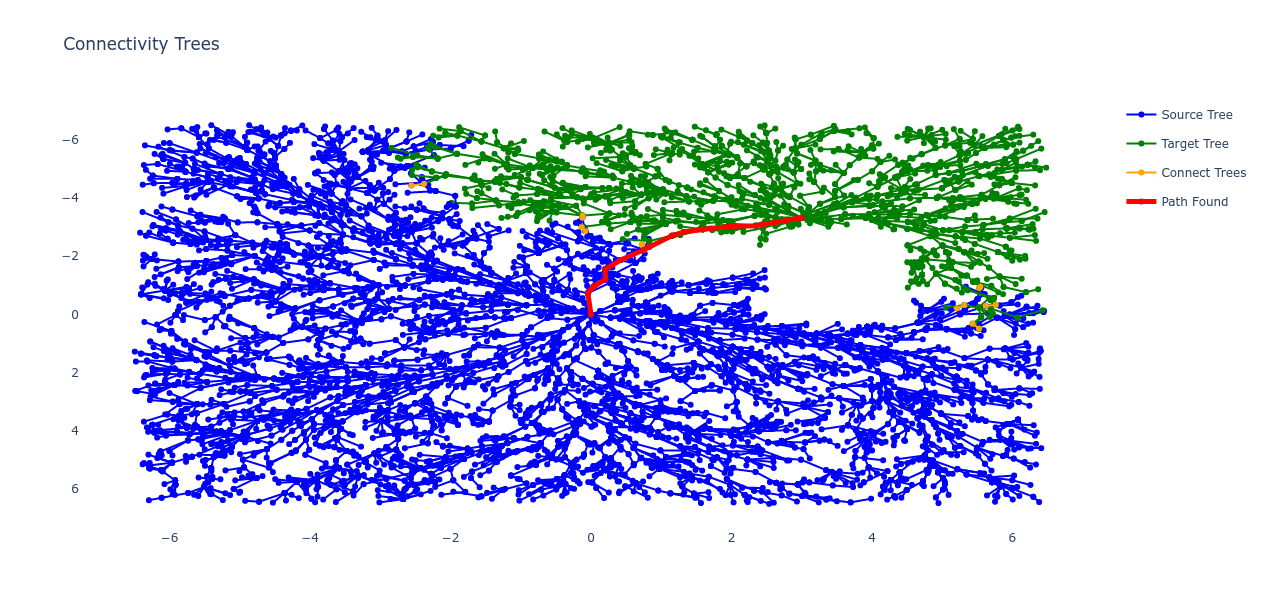
\includegraphics[width=1.1\textwidth]{figures/mp/mp_the_real_deal.png}
    \caption{A visualisation of the implemented \acs{RRT*} algorithm\\after a search from start to target}
    \end{subfigure}
    \label{fig:motion_planner_comparison}%
    \caption{Comparing schematic example to a visualisation of the real algorithm.}
\end{figure}

The result of adding an extra penalty for crossing unknown or movable subspace is that such subspaces are avoided if possible. If it is not possible to find a valid path, then movable or unknown subspaces are crossed, displayed in~\cref{fig:double_rrt_alg}. A path cannot be tracked by a controller if it crosses movable or unknown spaces, first the object must be moved, then the original path can be tracked. In~\cref{fig:double_rrt_alg} it can be seen that the motion planner cannot find a path around the movable object and is forced to add the cost to move the object. The added fixed cost for a path crossing through a movable or unknown objects motivates the motion planner to find the shortest path around objects but prefers moving an object over making a large detour.\bs

\begin{figure}[H]
    \centering
    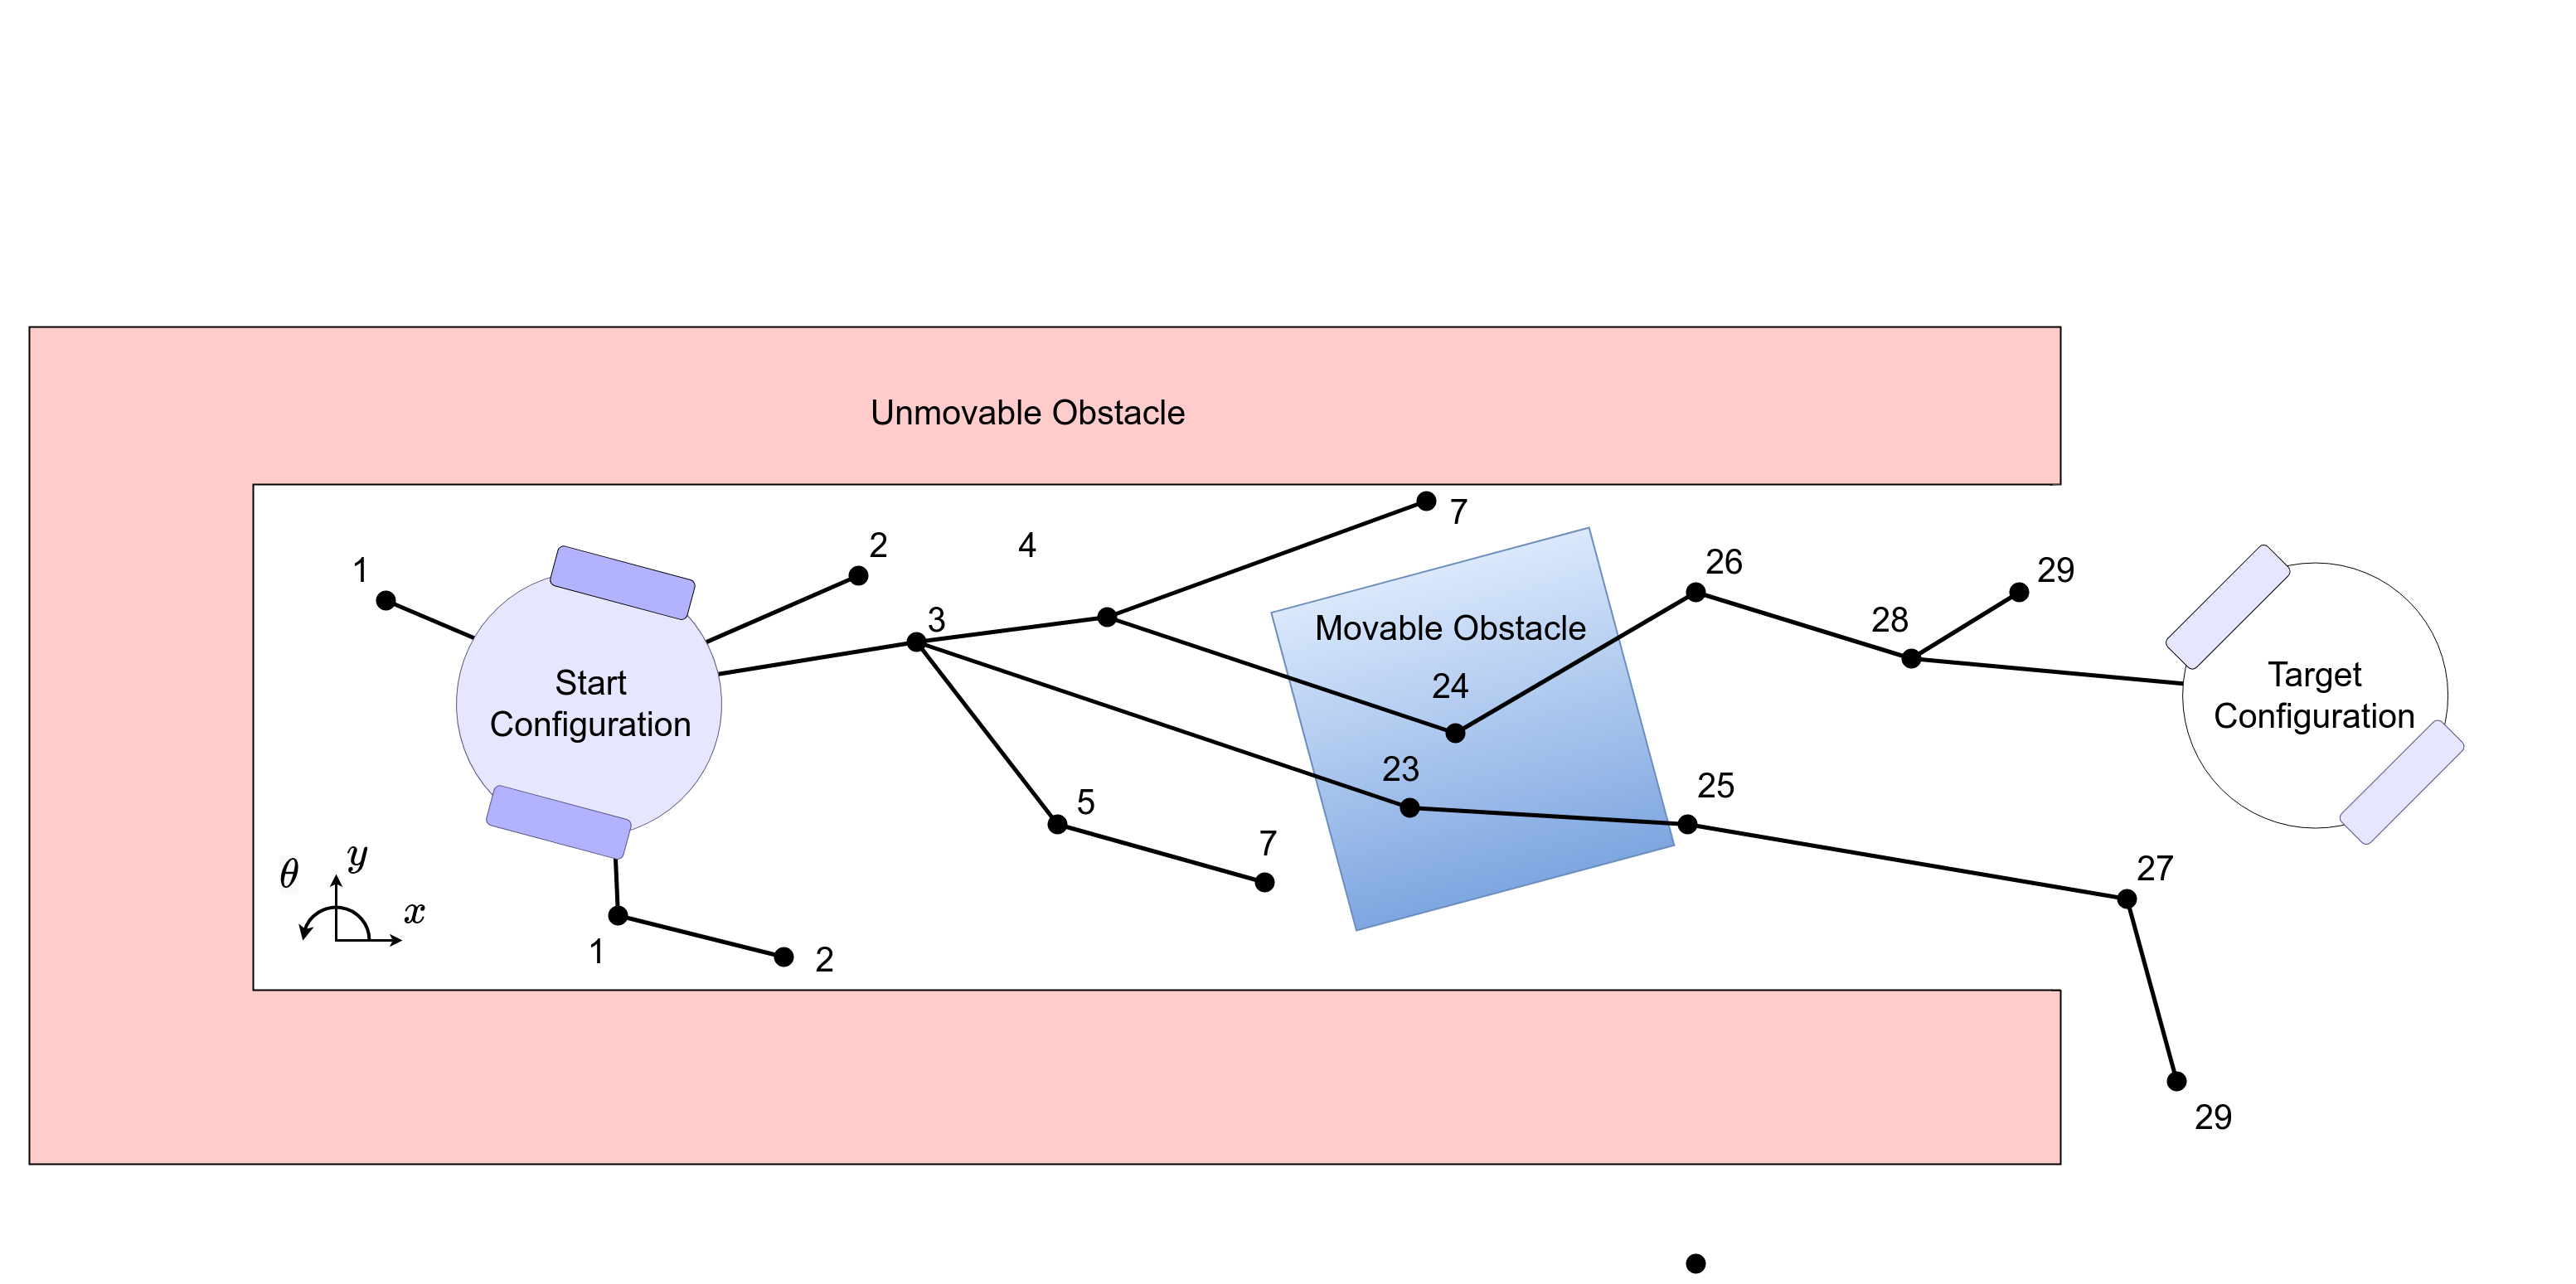
\includegraphics[width=0.9\textwidth]{figures/rrt_with_costs.png}
    \caption{Schematic view of the proposed double $\text{RRT}^*$ tree taking movable and\\unknown objects into account with cost to reach a sampled configuration displayed.}
    \label{fig:double_rrt_alg}
\end{figure}

The proposed motion planning algorithm searches the configuration space from from the start connectivity tree and the target connectivity tree. Exploring faster compared to the single tree \ac{RRT*} algorithm. The proposed algorithm rewires nodes, resulting in lowering the cost for existing paths. The proposed algorithm finds the optimal lowest cost path with infinite sampling because of it's ability to rewire nodes. The $LocalPlannerCheck$ provides paths which are feasible, such that the proposed algorithm yields paths that respect the system constraints. After all later on the system will be controlled to track the path. Now motion planning is discussed, manipulation will be discussed.


\subsection{Manipulation Planning}
\label{subsec:manipulation_planning}
\subsection{The Search and the Execution loop}
\label{subsec:2_loops}
\subsection{Fault Detection}
\label{subsec:fault_detection}
\subsection{Example}
\label{subsec:hgraph_example}

\section{Knowledge Graph}
\subsection{Definition}
\label{subsec:kgraph_definition}
\subsection{Edge Metrics}
\label{subsec:edge_metrics}
\subsection{Example}
\label{subsec:kgraph_example}
